

%*** General probabilistic notation ***

\newcommand{\expv}{\mathbf{E}} % EXP. VALUE
\newcommand{\discProbDist}{f} % Discrete prob distribution
\newcommand{\sampleSpace}{S} % Generic sample space
\newcommand{\sigmaAlg}{\mathcal{F}} % Generic sigma-algebra
\newcommand{\probm}{\mathbb{P}} % Generic probability measure, also prob. measure operator
\newcommand{\rvar}{X} % Generic random variable
%\newcommand{\dist}{\mathit{Dist}}

%*** MDP notation ***

\newcommand{\actions}{A} % The set of actions.
\newcommand{\colouring}{c} % the colouring function
\newcommand{\probTranFunc}{\Delta} % Transition function of an MDP
\newcommand{\edges}{E} % Set of edges in an MDP.
\newcommand{\colours}{C} % The set of colours in an MDP.
\newcommand{\mdp}{\mathcal{M}} % A generic MDP. 
\newcommand{\vinit}{v_0} % An initial vertex in an MDP.
\newcommand{\cylProb}{p} % Function assigning probabilities to cylinder sets in 
%the measure construction.
\newcommand{\emptyPlay}{\epsilon} %empty play
\newcommand{\objective}{\Omega} % Qualitative objective
\newcommand{\genColour}{\textsc{c}} % Generic colour
\newcommand{\quantObj}{f} % Generic quantitative objective
\newcommand{\indicator}[1]{\mathbf{1}_{#1}} % In.d RV
\newcommand{\eps}{\varepsilon} % Numerical epsilon
\newcommand{\maxc}{W} % Maximal abs. value of a colour

\newcommand{\winPos}{W_{>0}}
\newcommand{\winAS}{W_{=1}}
\newcommand{\cylinder}{\mathit{Cyl}}

\newcommand{\PrePos}{\text{Pre}_{>0}}
\newcommand{\PreAS}{\text{Pre}_{=1}}

\newcommand{\PreOPPos}{\mathcal{P}_{>0}}
\newcommand{\OPAS}{\mathcal{P}_{=1}}

\newcommand{\safeOP}{\mathit{Safe_{=1}}}
\newcommand{\closed}{\mathit{Cl}}

\newcommand{\reachOP}{\mathcal{V}}
\newcommand{\discOP}{\mathcal{D}}
\newcommand{\valsigma}{\vec{x}^{\sigma}}

\newcommand{\lp}{\mathcal{L}}
\newcommand{\lpdisc}{\lp_{\mathit{disc}}}
\newcommand{\lpmp}{\lp_{\mathit{mp}}}
\newcommand{\lpsol}[1]{\bar{#1}}
\newcommand{\lpmpdual}{\lpmp^{\mathit{dual}}}

\newcommand{\actevent}[3]{\actions^{#1}_{#2,#3}} % Returns #1-th action on the run 

\newcommand{\MeanPayoffSup}{\MeanPayoff^{+}}
\newcommand{\MeanPayoffInf}{\MeanPayoff^{-}}

\newcommand{\mcprob}{M}
\newcommand{\invdist}{\vec{z}}

\newcommand{\hittime}{T}



A possible taxonomy of algorithms for solving parity games distinguishes three families:
\begin{itemize}
	\item `strategy improvement algorithms', which construct a sequence of improving strategies until reaching an optimal strategy. 
	We will construct in \cref{3-sec:strategy_improvement} an exponential time strategy improvement algorithm.
	
	\item `attractor decomposition algorithms', which decompose a game through a sequence of attractor computations. 
	The first and archetypical example is McNaughton Zielonka algorithm defined in \cref{2-sec:parity}. 
	We will present in \cref{3-sec:zielonka} a quasipolynomial time algorithm improving over this algorithm.

	\item `value iteration algorithms', which find an optimal strategy through the computation of a value function.
	An equivalent point of view on this family of algorithms is the use of separating automata for reducing parity games to safety games.
	We introduce the framework of separating automata in \cref{3-sec:separation} and give a quasipolynomial time algorithm as an instanciation of it. 
	We then construct value iteration algorithms through the notion of universal trees in \cref{3-sec:value_iteration},
	and present a third quasipolynomial time algorithm in the form of a value iteration algorithm.
\end{itemize}

As a conclusion \cref{3-sec:relationships} discusses the relationships between the different algorithms: in what sense are separating automata and value iteration algorithms equivalent through the notion of universal trees, and how does this family compare to the other two families of algorithms described above.

\begin{remark}
We already proved in \cref{2-thm:parity} that parity games are positionally determined for both players, so in this chapter when considering a strategy we implicitly assume that it is positional.
\end{remark}

%%%%%%%%%%%%%%%%%%
%%%%%%%%%%%%%%%%%%
%%%%%%%%%%%%%%%%%%

\section{An exponential time strategy improvement algorithm}
\label{3-sec:strategy_improvement}
\begin{theorem}
\label{3-thm:strategy_improvement}
There exists a strategy improvement algorithm for solving parity games in exponential time.
\end{theorem}

We rely on the high-level presentation of strategy improvement algorithms given in \cref{1-sec:strategy_improvement}.
In a nutshell: the algorithm constructs a sequence of strategies, the next one being an improvement over the current one,
until reaching an optimal strategy.

\paragraph{\bf Adding the option of stopping the game.}
Let $\game$ a parity game with priorities in $[1,d]$.
Let us give Eve an extra move $\siblank$ that indicates that the game should stop and that she can play from any vertex of hers.
So a strategy for Eve is now a function $\sigma : \VE \rightarrow E \cup \set{\siblank}$ 
where $\sigma(v) = \siblank$ indicates that Eve has chosen to stop the game, and $\sigma(v) \ne \siblank$ should be interpreted as normal.
Adam is not allowed to stop the game, so strategies for Adam remain unchanged.
We say that a play ending with $\siblank$ is stopped.

For reasoning it will be useful to consider the parity graph $\Game[\sigma]$ obtained from $\Game$ by restricting the outgoing edges from $\VE$
to those prescribed by $\sigma$. 
Recall that we say that a parity graph (without stopping option) ""satisfies"" parity from $v$ if all infinite paths from $v$ satisfy parity.
Then a strategy $\sigma$ is winning from $v$ if and only if the parity graph $\Game[\sigma]$ satisfies parity from $v$.

Since we added the option for Eve to stop the game we introduce a new terminology: 
we say that a strategy $\sigma$ ""respects"" parity if all infinite plays consistent with $\sigma$ satisfy parity,
equivalently all infinite paths in $\Game[\sigma]$ satisfy parity, not requiring anything of stopped plays.

We say that a cycle is even if the maximal priority along the cycle is even, and it is odd otherwise. 
Respecting parity is characterised using cycles:
\begin{fact}
A strategy $\sigma$ ""respects"" parity if and only if all cycles in $\Game[\sigma]$ are even.
\end{fact}
The algorithm will only manipulate strategies respecting parity.

\paragraph{\bf Evaluating a strategy.}
The first question is: given a strategy $\sigma$, how to evaluate it (in order to later improve it)?
As explained in \cref{1-sec:strategy_improvement} towards this goal we define a value function $\val^{\sigma} : V \to Y$.

We let $\val^{\sigma}(v) = \min_\tau \val(\play_{\sigma,\tau}^v)$ where $\tau$ ranges over (general) strategies for Adam, so we first need to define the value of the play $\play = \play_{\sigma,\tau}^v$.
If $\play$ is stopped, then $\val(\play)$ is the tuple $(p_1, p_2, \dots, p_d)$ where $p_i$ is the number of times that priority $p$ appears on the play.
Otherwise $\val(\play)$ is $\top$ if $\play$ satisfies parity, and $\bot$ if $\play$ does not satisfy parity.
So the value of a play is either $\top$, $\bot$, or a multiset of priorities;
we let $Y$ denote the (infinite) set consisting of these elements.

We define a total order $\le$ on~$Y$ making it a complete lattice.
First, $\top$ is the greatest element and $\bot$ the least element.
For $t = (a_1, a_2, \dots, a_d)$ and $t' = (b_1, b_2, \dots, b_d)$,
we have that $t < t'$ if and only if $p$ is the largest index such that $t_p \ne t'_p$ and 
\begin{itemize}
	\item either $p$ is even and $t_p < t'_p$,
	\item or $p$ is odd and $t_p > t'_p$.
\end{itemize}
Then $\le$ is the reflexive closure of~$<$: we have $t \le t'$ if $t < t'$ or $t = t'$.

These conditions specify which priorities Eve likes to see along a play.
Given a choice, Eve would prefer to see even priorities and to avoid odd priorities, but these preferences are hierarchical: 
assuming that $d$ is even, Eve would like to see as many edges of priority $d$ as possible. 
If two plays see $d$ the same number of times, Eve prefers the play that visits the fewest vertices of
priority $d-1$, and if two plays see $d$ and $d-1$ the same number of times,
then Eve would like to maximise the number of times that $d-2$ is visited, and so on recursively.

\paragraph{\bf The value function as a fixed point.}
We define $\delta : Y \times [1,d] \to Y$ by 
\[
\delta(t,p) = 
\begin{cases}
(a_1, a_2, \dots, a_p + 1, a_{p+1}, \dots, a_d) & \text{ if } t = (a_1, a_2, \dots, a_d), \\
\top & \text{ if } t = \top, \\
\bot & \text{ if } t = \bot.
\end{cases}
\]
We note that $\delta$ is monotonic: for all $p \in [1,d]$,
if $t \le t'$ then $\delta(t,p) \le \delta(t',p)$. 
We extend $\delta$ to $\delta : Y \times [1,d]^* \to Y$.

We let $F^\sigma_V$ denote the set of functions $\mu : V \to Y$ such that $\mu(v) = \emptyset$ if $\sigma(v) = \siblank$,
it is a lattice when equipped with the componentwise (partial) order induced by $Y$:
we say that $\mu \le \mu'$ if for all vertices $v$ we have $\mu(v) \le \mu'(v)$.
We then define an operator $\Op : F^\sigma_V \to F^\sigma_V$ by
\[
\Op(\mu)(v) = 
\begin{cases}
\min \set{\delta( \mu(v'), \col(v)) : (v,v') \in E} & \text{if } \sigma(v) \neq \siblank \\
\emptyset 											& \text{if } \sigma(v) = \siblank.
\end{cases}
\]
Since $\delta$ is monotonic so is $\Op$.

\begin{fact}
The function $\val^\sigma$ is a fixed point of $\Op$ in $F^\sigma_V$.
\end{fact}
Unfortunately, $\val^{\sigma}$ is not in general the greatest fixed point of $\Op$ in $F^\sigma_V$;
let us analyse this in more details.
Let $\mu$ a fixed point of $\Op$ in $F^\sigma_V$, there are two cases. 
For a vertex $v$ such that there exists a stopped play $\pi$ starting from $v$, we have $\mu(v) \le \val(\pi)$, and more generally
$\mu(v) \le \inf_{\pi} \val(\pi)$ where $\pi$ ranges over all stopped plays starting from $v$.
The problem is for a vertex $v$ such that no plays starting from $v$ are stopped: 
we can have either $\mu(v) = \top$ or $\mu(v) = \bot$, irrespective of whether the play satisfies parity or not.
From this discussion we obtain the following result.

\begin{lemma}
\label{3-lem:greatest_fixed_point}
If $\sigma$ "respects" parity, then $\val^{\sigma}$ is the greatest fixed point of $\Op$ in $F^\sigma_V$.
\end{lemma}

\paragraph{\bf Improving a strategy.}
We reach the last item in the construction of the algorithm: the notion of switchable edges.
Let $\sigma$ a strategy. We say that an edge $e = (v,v')$ is switchable if 
\[
\delta(\val^{\sigma}(v'),\col(v)) > \delta(\val^{\sigma}(u),\col(v)) \text{ where } \sigma(v) = (v,u).
\]
Intuitively: according to $\val^{\sigma}$, playing $e$ is better than playing $\sigma(v)$.

Given a strategy $\sigma$ and an edge $e = (v,v')$ we use $\sigma[v \to e]$ to denote the strategy playing $e$ from $v$ 
and follow $\sigma$ from all other vertices.
Let us write $\sigma \le \sigma'$ if for all vertices~$v$ we have $\val^{\sigma}(v) \le \val^{\sigma'}(v)$,
and $\sigma < \sigma'$ if additionally $\neg (\sigma' \le \sigma)$.

\paragraph{\bf The algorithm.}
The algorithm starts with a specified initial strategy, which is the strategy
$\sigma_0$ where $\sigma_0(v) = \siblank$ for all vertices $v \in \VE$. 
It may not hold that $\sigma_0$ respects parity since $\game$ may contain odd cycles fully controlled by Adam.
This can be checked in linear time and the attractor to the corresponding vertices removed from the game.
After this preprocessing $\sigma_0$ indeed respects parity.

The pseudocode of the algorithm is given in \cref{3-algo:strategy_improvement}.
%The algorithm is the following: in each round $i$ compute $\val^{\sigma_i}$ and look for a switchable edge.
%If there exists a switchable edge $e_i = (v_i,p_i,v'_i)$, let $\sigma_{i+1} = \sigma_i[v_i \to e_i]$ and iterate to the next round.
%Otherwise, return the strategy $\sigma_i$.

\begin{algorithm}
 \KwData{A parity game $\game$}
 \SetKwBlock{Repeat}{repeat}{}
 \DontPrintSemicolon
 
 $i \leftarrow 0$
 
 \For{$v\in \VE$}{
   $\sigma_0(v) \leftarrow \siblank$
 }

 $C \leftarrow \set{v \in V : v \text{ contained in an odd cycle in } \game[\sigma_0]}$

 $\Game \leftarrow \Game \setminus \AttrA(C)$
 
 \Repeat{
   Compute $\val^{\sigma_i}$ 

	\If{$\exists e_i = (v_i,v'_i) \in E \text{ switchable}$}{
		$\sigma_{i+1} \leftarrow \sigma_i[v_i \to e_i]$
		
		$i \leftarrow i + 1$

	} 
	\Else{
		\Return{$\set{v \in V : \val^{\sigma_i}(v) = \top}$}
	}
 }

 \caption{The strategy improvement algorithm for parity games.}
\label{3-algo:strategy_improvement}
\end{algorithm}

%Note that one cannot start the algorithm with an arbitrary strategy, since if we happen to pick a
%strategy $\sigma$ that allows Adam to win everywhere, then all vertices will
%have value $\bot$, and there will be no switchable edges. However, if we
%start with a strategy where all vertices have a value that is not $\bot$,
%then we can never reach a strategy where any vertex has value $\bot$.

\paragraph{\bf Proof of correctness.}
We start by stating a very simple property of $\delta$, which is key in the arguments below.

\begin{fact}
Let $t \in Y$ and $p_1,\dots,p_k \in [1,d]$ such that $t$ and $\delta(t,p_1 \dots p_k)$ are neither $\top$ nor $\bot$.
Then $t \le \delta(t,p_1 \dots p_k)$ if and only if $\max \set{p_1,\dots,p_k}$ is even.
\end{fact}

The following lemma states the two important properties of $(Y,\le)$ and $\delta$.

\begin{lemma}
\label{3-lem:key_property}
Let $G$ a parity graph (with no stopping option).
\begin{itemize}
	\item If there exists $\mu : V \to Y$ such that for all vertices $v$ we have $\mu(v) \neq \top,\bot$
	and for all edges $(v,u) \in E$ we have $\mu(v) \le \delta(\mu(u),\col(v))$,
	then $G$ satisfies parity.
	\item If there exists $\mu : V \to Y$ such that for all vertices $v$ we have $\mu(v) \neq \top,\bot$
	and for all edges $(v,u) \in E$ we have $\mu(v) \ge \delta(\mu(u),\col(v))$,
	then $G$ satisfies the complement of parity.
\end{itemize}
\end{lemma}
\begin{proof}
We prove the first property, the second is proved in exactly the same way.
Thanks to the characterisation using cycles it is enough to show that all cycles in $G$ are even.
Let us consider a cycle in $G$:
\[
\pi = (v_0,v_1) (v_1,v_2) \cdots (v_{k-1},v_0).
\]
For all $i \in [0,k-1]$ we have $\mu(v_i) \le \delta(\mu(v_{i+1 \mod k}),\col(v_i))$.
By monotonicity of $\delta$ this implies $\mu(v_1) \le \delta(\mu(v_1),\col(v_{k-1}) \cdots \col(v_0))$.
Thanks to \cref{3-lem:key_property} this implies that the maximum priority in $\set{\col(v_0),\dots,\col(v_{k-1})}$ is even.
\end{proof}

Let $\sigma$ a strategy respecting parity. 
A progress measure for $\Game[\sigma]$ is a post-fixed point of $\Op$ in $F^\sigma_V$:
it is a function $\mu : V \to Y$ such that $\mu(v) = \emptyset$ if $\sigma(v) = \siblank$ and $\mu \le \Op(\mu)$,
which means that $\mu(v) \le \min \set{ \delta(\mu(v'),\col(v)) : (v,v') \in E}$.

We now rely on \cref{3-lem:greatest_fixed_point} and \cref{3-lem:key_property} to prove the two principles: progress and optimality.

\begin{lemma}[Progress]
Let $\sigma$ a strategy respecting parity and $e = (v,v')$ a switchable edge.
We let $\sigma'$ denote $\sigma[v \to e]$.
Then $\sigma'$ respects parity and $\sigma < \sigma'$.
\end{lemma}

\begin{proof}
We first argue that $\sigma'$ respects parity.
The fact that $e = (v,v')$ is switchable reads
\[
\delta(\val^\sigma(v'),\col(v)) > \delta(\val^\sigma(u),\col(v)),
\]
and by definition of $\val^\sigma$ we have $\val^\sigma(v) = \delta(\val^\sigma(u),\col(v))$,
which implies $\val^\sigma(v) < \delta(\val^\sigma(v'),\col(v))$, and in particular $\val^\sigma(v) \neq \top$.

Let us consider the parity graph $\Game[\sigma']$ and note that for all edges $e' = (s,t)$ 
we have $\val^\sigma(s) \le \delta(\val^\sigma(t),\col(s))$:
indeed either $e'$ is an edge in $\Game[\sigma]$ and this is by definition of $\val^\sigma$,
or $e' = e$ and the inequality was proved just above.

Since $\sigma$ respects parity $\val^\sigma$ does not take the value $\bot$.
But we cannot apply (the first item of) \cref{3-lem:key_property} yet because $\val^\sigma$ may have value $\top$.
However by definition of $\val^\sigma$ for all vertices $s$ such that $\val^\sigma(s) = \top$ all paths from $s$ satisfy parity,
so it is enough to consider the parity graph obtained from $\Game[\sigma']$ by removing all such vertices.
The first item of \cref{3-lem:key_property} implies that it satisfies parity, hence $\Game[\sigma']$ as well.

\vskip1em
At this point we know that $\sigma'$ respects parity, which thanks to \cref{3-lem:greatest_fixed_point}
implies that $\val^{\sigma'}$ is the greatest fixed point of $\Op$ in $F^{\sigma'}_V$.

We now argue that $\val^\sigma$ is a progress measure for $\game[\sigma']$.
For all vertices but $v$ this is clear because the outgoing edges are the same in $\game[\sigma]$ and in $\game[\sigma']$.
For $v$ as argued above we have $\val^\sigma(v) < \delta(\val^\sigma(v'),\col(v))$.
It follows that $\val^\sigma$ is indeed a progress measure for $\game[\sigma']$.
Since $\val^{\sigma'}$ is the greatest fixed point of $\Op$ in $F^{\sigma'}_V$, this implies that 
$\val^{\sigma} \le \val^{\sigma'}$.

We now show that $\val^{\sigma} < \val^{\sigma'}$. 
Using $\val^{\sigma}(v') \le \val^{\sigma'}(v')$ and the monotonicity of $\delta$ we obtain that
$\delta(\val^\sigma(v'),\col(v)) \le \delta(\val^{\sigma'}(v'),\col(v))$.
By definition of $\val^{\sigma'}$ we have $\val^{\sigma'}(v) = \delta(\val^{\sigma'}(v'),\col(v))$
and together with $\val^\sigma(v) < \delta(\val^\sigma(v'),\col(v))$ this implies that
$\val^\sigma(v) < \val^{\sigma'}(v)$.
\end{proof}

\begin{lemma}[Optimality]
Let $\sigma$ a strategy respecting parity that has no switchable edges, then 
$\sigma$ is winning from all vertices of $\WE(\Game)$.
\end{lemma}

\begin{proof}
The fact that $\sigma$ respects parity means that it is a winning strategy
from all vertices $v$ such that $\val^\sigma(v) = \top$.
It also implies that for all vertices $v$ we have $\val^{\sigma}(v) \neq \bot$.
We now prove that Adam has a winning strategy from all vertices $v$ such that $\val^{\sigma}(v) \neq \top$.
We construct a strategy of Adam by
\[
\forall v \in \VA,\ \tau(v) = \argmin \set{ \delta(\val^{\sigma}(u),\col(v)) : (v,u) \in E }.
\]
We argue that $\tau$ ensures the complement of parity from all vertices $v$ such that $\val^{\sigma}(v) \neq \top$.
Let us consider $\Game[\tau]$ the parity graph obtained from $\Game$ by restricting the outgoing edges from $\VA$
to those prescribed by $\tau$.
We argue that for all edges $(v,,v')$ in $\game[\tau]$, we have 
$\val^{\sigma}(v) \ge \delta(\val^{\sigma}(v'),\col(v))$.
Once this is proved we conclude using the second item of \cref{3-lem:key_property} implying that $\Game[\tau]$ satisfies the complement of parity.

The first case is when $v \in \VE$. 
Let $\sigma(v) = (v,u)$.
Since the edge $e = (v,v')$ is not switchable we have 
$\delta(\val^{\sigma}(v'),\col(v)) \le \delta(\val^{\sigma}(u),\col(v))$.
By definition of $\val^\sigma$ we have $\val^\sigma(v) = \delta(\val^{\sigma}(u),\col(v))$,
implying the desired inequality.

The second case is when $v \in \VA$, it holds by definition of $\tau$.
\end{proof}

\paragraph{\bf Complexity analysis.}
The computation of $\val^\sigma$ for a strategy $\sigma$ can be seen to be a shortest path problem where distances are measured using the operator $\le$. 
Thus, any algorithm for the shortest path problem can be applied, such as the Bellman-Ford algorithm.
In particular computing $\val^\sigma$ can be done in polynomial time, and even more efficiently through a refined analysis.

An aspect of the algorithm we did not develop is choosing the switchable edge.
It is possible to switch not only one edge but a set of switchable edges at each iteration, making this question worse: 
which subset of the switchable edges should be chosen?
Many possible rules for choosing this set have been studied, as for instance the \emph{greedy all-switches} rule. 

The next question is the number of iterations, meaning the length of the sequence
$\sigma_0,\sigma_1,\dots$. It is at most exponential since it is bounded by the number of strategies (which is bounded aggressively by $m^n$).
There are lower bounds showing that the sequence can be of exponential length, which apply to different rules for choosing switchable edges.
Hence the overall complexity is exponential; we do not elaborate further here. 
%We refer to \cref{3-sec:references} for bibliographic references and a discussion on the family of strategy improvement algorithms.


%%%%%%%%%%%%%%%%%%
%%%%%%%%%%%%%%%%%%
%%%%%%%%%%%%%%%%%%

\section{A quasipolynomial time attractor decomposition algorithm}
\label{3-sec:zielonka}
The Zielonka tree is a combinatorial structure associated with a Muller objective which very neatly exposes its properties.
As a warm-up we first present its predecessor the LAR construction, and then show the properties of Zielonka trees.
As we will see, the key feature of the Zielonka tree of a Muller objective $\Muller(\F)$ is to characterise its exact memory requirements.

\subsection*{The latest appearance record}
Muller objectives can be reduced to parity objectives, see~\cref{1-sec:reductions} for an introduction to reductions between objectives.

\begin{theorem}
\label{2-thm:LAR}
Let $C = [1,d]$ be a set of colours and $\Muller(\F)$ a Muller objective.
There exists a deterministic parity automaton $\LAR_\F$ over the alphabet $C$ defining $\Muller(\F)$.
It has $d!$ states and has priorities in $[1,2d]$.
\end{theorem}

LAR stands for ""Latest Appearance Record"".
In the literature the number of states is often $d \cdot d!$ instead of $d!$,
the multiplicative factor $d$ is saved since for automata the acceptance conditions are transition based 
instead of state based.

\begin{proof}
We define the automaton $\LAR_\F$.
The set of states is the set of lists of all colours of $C$ without repetitions.
We represent a list by $(c_1,\dots,c_d)$.
The initial state is irrelevant because $\Muller(\F)$ is prefix independent.
The transition function is defined as follows: 
$\delta(\ell, c)$ is $\ell'$ obtained from $\ell$ by pushing $c$ to the first position (hence shifting to the right the elements to the left of $c$). 
This is best understood on an example: 
\[
\delta( (4, 1, 2, 3), 2) = (2, 4, 1, 3).
\]
Let $j$ be the position of $c$ in $\ell$, the priority of this transition is defined by:
\[
\col((\ell,c,\ell')) =
\begin{cases}
2 j      & \text{ if } \ell([1,j]) \in \F, \\
2 j - 1  & \text{ otherwise.}
\end{cases}
\]

We now show that the automaton $\LAR_\F$ defines $\Muller(\F)$.
Let $\rho = c_0 c_1 \dots$ be an infinite word over the alphabet $C$. 
Let us consider the run of $\LAR_\F$ over~$\rho$:
\[
(\ell_0,c_0,\ell_1) (\ell_1,c_1,\ell_2) \dots
\]
Let us write $j_i$ for the position of $c_i$ in $\ell_i$.
We consider $\Inf(\rho)$ the set of colours appearing infinitely many times and write $j$ for its cardinal.
From some point onwards the lists $\ell_i$ are of the form 
\[
(\underbrace{c_1,\dots,c_j}_{\Inf(\rho)} ,\ \underbrace{c_{j + 1},\dots,c_d}_{C \setminus \Inf(\rho)}).
\]
From this point on $j_i$ is smaller than or equal to $j$, and it reaches $j$ infinitely many times.
It follows that the largest priority appearing infinitely many times in the run is $2 j$ if $\Inf(\rho) \in \F$
and $2 j - 1$ if $\Inf(\rho) \notin \F$.
Thus $\rho$ is accepted by $\LAR_\F$ if and only if $\Inf(\rho) \in \F$, as desired.
%The set of states is the set of lists of all colours of $C$ without repetitions and with a marked position.
%We represent a list by $(c_1,\dots,\overline{c_j},\dots,c_d)$: the marked position is $j$.
%The initial state is irrelevant because $\Muller(\F)$ is prefix independent.
%The transition function is defined as follows: 
%$\delta(\ell, c)$ is $\ell'$ obtained from $\ell$ by pushing $c$ to the first position 
%(hence shifting to the right the elements to the left of $c$)
%and marking the position of $c$ in $\ell$.
%This is best understood on an example: 
%\[
%\delta( (4, 1, 2, \overline{3}), 2) = (2, 4, \overline{1}, 3).
%\]
%The prioritiy is the list $\ell$ with a marked position $j$ is defined by:
%\[
%\col((\ell,j)) =
%\begin{cases}
%2 j      & \text{ if } \ell([1,j]) \in \F, \\
%2 j - 1  & \text{ otherwise.}
%\end{cases}
%\]
%We now show that the automaton $\LAR_\F$ defines $\Muller(\F)$.
%Let $\rho = c_0 c_1 \dots$ be an infinite word over the alphabet $C$. 
%Let us consider the run $\ell_0 \ell_1 \dots$ of $\LAR_\F$ over~$\rho$
%and write $j_i$ for the marked position of $c_i$ in $\ell_i$.
%We consider $\Inf(\rho)$ the set of colours appearing infinitely many times and write $j$ for its cardinal.
%From some point onwards the lists $\ell_i$ are of the form 
%\[
%(\underbrace{c_1,\dots,c_j}_{\Inf(\rho)} ,\ \underbrace{c_{j + 1},\dots,c_d}_{C \setminus \Inf(\rho)}).
%\]
%From this point on $j_i$ is smaller than or equal to $j$, and it reaches $j$ infinitely many times.
%It follows that the largest priority appearing infinitely many times in the run is $2 j$ if $\Inf(\rho) \in \F$
%and $2 j - 1$ if $\Inf(\rho) \notin \F$.
%Thus $\rho$ is accepted by $\LAR_\F$ if and only if $\Inf(\rho) \in \F$, as desired.
\end{proof}

\subsection*{The Zielonka tree}
\Cref{2-thm:LAR} implies a reduction from Muller games to parity games as explained in \cref{1-sec:reductions}.
However this does not improve over the results we already obtained for Muller games in \cref{2-thm:muller},
neither algorithmically nor for the memory requirements.
One weakness of the LAR construction is that its size depends only on the number of colours, and not on the properties of $\F$.
The Zielonka tree is an improved take on the "LAR".

\begin{definition}[Zielonka tree]
\label{definition:zielonka_tree}
Let $\Muller(\F)$ be a Muller objective over the set of colours $C$.
The Zielonka tree $T_\F$ of $\Muller(\F)$ is a rooted tree with nodes labelled by subsets of colours, 
it is constructed inductively as follows:
\begin{itemize}
	\item the root is labelled $C$,
	\item the children of a node labelled $S$ are the maximal subsets $S_1, \dots, S_k$ of $S$ such that 
	$S_i \in \Muller(\F) \Longleftrightarrow S \notin \Muller(\F)$.
\end{itemize}
\end{definition}

%A Muller objective where each of $n$ colours have to be visited infinitely often (sometimes called a generalized B\"uchi objective) can be solved in polynomial time, but the "LAR" reduction would still involve a $d!$ blowup in the number of states.

\cref{2-fig:Zielonka_tree_example} represents the Zielonka tree for $\Muller(\F)$ with 
\[
\F = \set{\set{2}, \set{3}, \set{4}, \set{1,2}, \set{1,3}, \set{1,3,4}, \set{2,3,4}, \set{1,2,3,4}}.
\]
We note that there are two nodes labelled $\set{1}$; in general there may be several nodes with the same label.
Also, not all branches have the same length.
%The definition of the Zielonka tree can be refined into the Zielonka DAG (directly acyclic graph).

\begin{figure}
\centering
  \begin{tikzpicture}[scale=1.1]
\node[s-eve, dashed] (1234) at (5,3.5) {$\ \set{1,2,3,4}\ $};

\node[s-adam, dashed] (123) at (2,2) {$\ \set{1,2,3}\ $};
\node[s-eve] (12g) at (1,1) {$\ \set{1,2}\ $};
\node[s-adam] (1g) at (1,0) {$\ \set{1}\ $};
\node[s-eve, dashed] (13) at (3,1) {$\ \set{1,3}\ $};
\node[s-adam, dashed] (1m) at (3,0) {$\ \set{1}\ $};

\node[s-adam] (124) at (5,2) {$\ \set{1,2,4}\ $};
\node[s-eve] (12d) at (4,1) {$\ \set{1,2}\ $};
\node[s-adam] (1d) at (4,0) {$\ \set{1}\ $};
\node[s-eve] (4g) at (6,1) {$\ \set{4}\ $};

\node[s-adam] (34) at (8,2) {$\ \set{3,4}\ $};
\node[s-eve] (3) at (7,1) {$\ \set{3}\ $};
\node[s-eve] (4d) at (9,1) {$\ \set{4}\ $};

\node (l1) at (10,0) {$\ 1\ $};
\node (l2) at (10,1) {$\ 2\ $};
\node (l3) at (10,2) {$\ 3\ $};
\node (l4) at (10,3.5) {$\ 4\ $};

% create edges
\path
  (1234) edge (123)
  (1234) edge (124)
  (1234) edge (34)
  (123) edge (12g)
  (12g) edge (1g)
  (123) edge (13)
  (13) edge (1m)
  (124) edge (12d)
  (124) edge (4g)
  (12d) edge (1d)
  (34) edge (3)
  (34) edge (4d);  
  \end{tikzpicture}
\caption{The Muller tree for $\Muller(\F)$. By convention nodes labelled by a set in $\F$ are represented by a circle
and the others by a square.
The numbers on the right hand side and the dashed nodes (describing a branch) are both used in the proof of \cref{2-thm:reduction_parity_Zielonka_tree}.}
\label{2-fig:Zielonka_tree_example}
\end{figure}

The first use of the Zielonka tree is to induce an improved reduction from Muller to parity objectives.
A branch in a tree is a path from the root to a leaf.

\begin{theorem}
\label{2-thm:reduction_parity_Zielonka_tree}
Let $C = [1,d]$ be a set of colours and $\Muller(\F)$ a Muller objective.
There exists a deterministic parity automaton $\Zielonka_\F$ over the alphabet $C$ defining $\Muller(\F)$.
Its number of states is the number of branches of $T_\F$ and its parity condition uses $d$ priorities.
\end{theorem}

Here again we take advantage of the fact that the acceptance conditions on automata are transition based;
using stated based transitions we would have add a multiplicative factor $d$.

\begin{proof}
Without loss of generality $C \in \F$ (otherwise we consider the complement $\Muller(2^C \setminus \F)$).
We number the levels of $T_\F$ from the leaves to the root such that nodes labelled by sets in $\F$ are even
and the other ones odd (this will be used for defining the parity condition).
See \cref{2-fig:Zielonka_tree_example} for a possible numeration of the levels (on the right hand side), the other options being shifts of this numeration by an even number.

The set of states of $\Zielonka_\F$ is the set of branches of $T_\F$.
We represent a branch by $(S_1,\dots,S_k)$
where $S_1$ is the set labelling the root and $S_k$ the set labelling a leaf. Note that $k \le d$.
For the sake of simplicity we identify nodes with their labels, which is an abuse since two different nodes may have the same label
but will be convenient and harmless in our reasoning.

The initial state is irrelevant because $\Muller(\F)$ is prefix independent.
We define the support $\support(b,c)$ of a branch $b$ and a colour $c$ to be the lowest node of $b$ which contains~$c$.
The transition function is defined as follows: 
$\delta(b,c)$ is the next branch (in the lexicographic order from left to right and in a cyclic way) which coincides with $b$ up to $\support(b,c)$.
The priority of this transition is given by the level on which $\support(b,c)$ sits.

This is best understood on an example: on \cref{2-fig:Zielonka_tree_example}
consider the branch $b$ represented by dashed nodes, reading the colour $2$ we consider branches starting with $(\set{1,2,3,4}, \set{1,2,3})$
because $\support(b,2) = \set{1,2,3}$.
The next branch after $b$ is $(\set{1,2,3,4}, \set{1,2,3},\set{1,2},\set{1})$ (because we cycle: the node after $\set{1,3}$ is $\set{1,2}$).
The priority of this transition is $3$ corresponding to the level where $\set{1,2,3}$ sits.

We now show that the automaton $\Zielonka_\F$ defines $\Muller(\F)$.
Let $\rho = c_0 c_1 \dots$ be an infinite word over the alphabet $C$.
Let us consider the run of $\Zielonka_\F$ over~$\rho$:
\[
(b_0,c_0,b_1) (b_1,c_1,b_2) \dots
\]
We consider $\Inf(\rho)$ the set of colours appearing infinitely many times.
Let us look at the largest prefix $(S_1,\dots,S_p)$ of a branch which is eventually common to all the branches $b_i$.
We make two claims:
\begin{itemize}
	\item $\Inf(\rho)$ is included in $S_p$;
	\item $\Inf(\rho)$ is not included in any child of $S_p$.
\end{itemize}
For the first claim, let $c \in \Inf(\rho)$, since eventually the branch $b_i$ starts with $(S_1,\dots,S_p)$,
the support of $b_i$ and $c$ is lower than or equal to $S_p$, meaning that $c \in S_p$.

For the second claim, we first note that by maximality of $(S_1,\dots,S_p)$ the support of $b_i$ and $c_i$ is infinitely many times $S_p$.
Indeed from some point onwards it is lower than or equal to $S_p$, and if it would be eventually strictly lower then the corresponding child of $S_p$ would be common to all branches $b_i$ from there on.
This implies that all children of $S_p$ appear infinitely many times in the branches $b_i$: each time the support of $b_i$ and $c_i$ is $S_p$, the branch switches to the next child of $S_p$.
Now since each child $S_{p+1}$ of $S_p$ is left infinitely many times this implies that there exists $c \in \Inf(\rho)$ with $c \notin S_{p+1}$.
Hence $\Inf(\rho)$ is not included in $S_{p+1}$.

By definition of the Zielonka tree, this implies that $\Inf(\rho) \in \F$ if and only if $S_p \in \F$,
thus $\rho$ is accepted by $\Zielonka_\F$ if and only if $\Inf(\rho) \in \F$, as desired.
\end{proof}

Since \cref{2-thm:reduction_parity_Zielonka_tree} is a reduction from Muller to parity objectives,
it implies a reduction from Muller games to parity games as explained in \cref{1-sec:reductions},
improving over \cref{2-thm:LAR}. 
Since solving parity games is in $\NP \cap \coNP$,
if we represent the Muller condition by a Zielonka tree then the automaton constructed in \cref{2-thm:reduction_parity_Zielonka_tree}
is of polynomial size, implying the following result.

\begin{theorem}
Solving Muller games where the condition is represented by a Zielonka tree is in $\NP \cap \coNP$.
\end{theorem}

As observed above different nodes of the Zielonka tree may be labelled by the same set of colours.
Hence it is tempting to represent a Muller condition not with its Zielonka tree but rather with the Zielonka DAG (Directed Acyclic Graph)
where nodes labelled by the same set of colours are identified.
However with this representation solving Muller games is again $\PSPACE$-complete:

\begin{theorem}
\label{2-thm:Muller_games_DAG}
Solving Muller games where the condition is represented by a Zielonka DAG is $\PSPACE$-complete.
\end{theorem}

The algorithm presented in \cref{2-thm:muller} runs in polynomial space for this representation.
To obtain the $\PSPACE$-hardness we observe that in the reduction from QBF constructed in \cref{2-thm:complexity_Muller},
the Muller objective is of polynomial size when represented by a Zielonka DAG (but of exponential size when represented by a Zielonka tree).

\subsection*{The exact memory requirements}
The second and most interesting use of the Zielonka tree is for characterising the memory requirements.

Note that a node in the Zielonka tree $T_\F$ represents another Muller objective, over the set of colours labelling this node.
For instance in \cref{2-fig:Zielonka_tree_example} the node labelled $\set{1,2,3}$ corresponds to $\Muller(\F')$ with
$\F' = \set{\set{2}, \set{3}, \set{1,2}, \set{1,3}}$.

\begin{definition}
Let $\Muller(\F)$ be a Muller objective over the set of colours $C$.
We define $m_\F$ by induction:
\begin{itemize}
	\item if the tree consists of a single leaf, then $m_\F = 1$;
	\item otherwise, let $\F_1,\dots,\F_k$ be the Muller objectives defined by the children of the root,
	there are two cases:
	\begin{itemize}
		\item if $C \in \F$, then $m_\F$ is the \textit{sum} of $m_{\F_1},\dots,m_{\F_k}$;
		\item if $C \notin \F$, then $m_\F$ is the \textit{maximum} of $m_{\F_1},\dots,m_{\F_k}$.
	\end{itemize}
\end{itemize}
\end{definition}

For the Muller objective represented in \cref{2-fig:Zielonka_tree_example}, we have $m_\F = 3$.
In the following result we consider \textit{partial} colouring functions: $\col : V \to C \cup \set{\emptyset}$,
meaning that some vertices can be left uncolored (formally, labelled $\emptyset$).

\begin{theorem}
\label{2-thm:characterisation_Zielonka_tree}
Muller objectives $\Muller(\F)$ are determined with finite memory strategies of size $m_\F$
for games with \textit{partial colouring functions}\footnote{See \cref{2-rmk:finite_infinite} for the case of infinite games.}.
This bound is tight: there exists a game with objective $\Muller(\F)$ where Eve wins using $m_\F$ memory states
but not with less.
\end{theorem}

Let us show on an example that the assumption of partial colouring functions is necessary.
Let $\F = \set{ \set{1,2} }$: the objective $\Muller(\F)$ requires that both $1$ and $2$ are seen infinitely many times.
The Zielonka tree $T_\F$ has three nodes $\set{1,2}, \set{1}$, and $\set{2}$, and $m_\F = 2$.
Indeed $\Muller(\F)$ is determined with finite memory strategies of size $2$:
intuitively the memory structure is used to remember which colour was last seen.
A game with a partial colouring function where two memory states is necessary is presented in~\cref{2-fig:lower_bound_zielonka}.
However, $\Muller(\F)$ is positionally determined for games with total colouring functions (as we have defined them originally):
intuitively since every vertex has colour either $1$ or $2$, there is no need to remember which colour was last seen.

\begin{figure}
\centering
  \begin{tikzpicture}[scale=1.3]
    \node[s-eve] (v0) at (2,0) {$\begin{array}{c} v_1 \\ \ \end{array}$};
    \node[s-eve] (v1) at (0,0) {$\begin{array}{c} v_0 \\ 1 \end{array}$};
    \node[s-eve] (v2) at (4,0) {$\begin{array}{c} v_2 \\ 2 \end{array}$};
    % create edges
    \path[arrow]
      (v0) edge[bend left] (v1)
      (v1) edge[bend left] (v0)
      (v0) edge[bend left] (v2)
      (v2) edge[bend left] (v0);
  \end{tikzpicture}
\caption{A game with a partial colouring function 
where Eve has a winning strategy for $\Muller(\F)$ with $\F = \set{ \set{1,2} }$ using two memory states
but no positional winning strategy.}
\label{2-fig:lower_bound_zielonka}
\end{figure}




We will not construct the lower bound, meaning the game where Eve needs $m_\F$ memory states to win.
However, we will now prove the upper bound.
To this end we revisit the recursive algorithm presented in \cref{2-lem:Muller_even} and \cref{2-lem:Muller_odd}.
This algorithm was removing colours one by one and rely on the recursive solutions.
We show that we can adapt the algorithm to follow instead the structure of the Zielonka tree: 
for solving a Muller game, it is enough to recursively solve the induced Muller games
corresponding to the children of the root of the Zielonka tree.
The following lemma is an improved variant of \cref{2-lem:Muller_even}.

\begin{lemma}\label{2-lem:McNaughton_Zielonka_even}
Let $\Game$ be a Muller game with objective $\Muller(\F)$ such that $C \in \F$.
Let $C_1, \dots, C_k$ be the maximal subsets of $C$ such that $C_i \notin \F$.
We let $\F_1,\dots,\F_k$ be the corresponding induced Muller objectives,
and define $\Game_i$ be the subgame of $\Game$ induced by $V \setminus \AttrE(C \setminus C_i)$
with objective $\Muller(\F_i)$.
\begin{itemize}
	\item If for all $i \in [1,k]$, we have $\WA(\Game_i) = \emptyset$, then $\WE(\Game) = V$.
	\item If there exists $i \in [1,k]$ such that $\WA(\Game_i) \neq \emptyset$,
	let $\Game'$ be the subgame of $\Game$ induced by $V \setminus \AttrA( \WA(\Game_i) )$,
	then $\WE(\Game) = \WE(\Game')$.
\end{itemize}
\end{lemma}

We will prove the memory requirement at the same time inductively.
Note that by duality, the case where $C \notin \F$ corresponds to the memory requirement for Adam when $C \in \F$:
\[
m_{2^C \setminus \F} = \max_{i \in [1,k]} m_{2^{C_i} \setminus \F_i}.
\]

\begin{proof}
We prove the first item.

For each $i \in [1,k]$, let $\sigma_i$ be an attractor strategy ensuring to reach $C_i$ from $\AttrE(C_i)$,
and consider a winning strategy for Eve from $V \setminus \AttrE(C_i)$ in $\Game_i$, it induces a strategy $\sigma'_i$ in $\Game$.
We construct a strategy $\sigma$ in $\Game$ which will simulate the strategies above in turn; to do so it uses $[1,k]$ as top-level memory states.
(We will look at more closely at the memory structure at the end of the proof.)
The strategy $\sigma$ with memory $i$ simulates $\sigma_i$ from $\AttrE(C_i)$ and $\sigma'_i$ from $V \setminus \AttrE(C_i)$,
and if it ever reaches a vertex in $C_i$ it updates its memory state to $i + 1$ and $1$ if $i = k$.
Any play consistent with $\sigma$ either updates its memory state infinitely many times, 
or eventually remains in $V \setminus \AttrE(C_i)$ and is eventually consistent with $\sigma'_i$.
In the first case it sees a colour from each $C_i$ infinitely many times, so by definition of the $C_i$'s and since $C \in \F$ 
the play satisfies $\Muller(\F)$, 
and in the other case since $\sigma'_i$ is winning the play satisfies $\Muller(\F)$.
Thus $\sigma$ is winning from $V$.

Let us now discuss how many memory states are necessary to implement the strategy $\sigma$.
By induction hypothesis, each of the strategies $\sigma'_i$ uses $m_{\F_i}$ memory states.
Using a disjoint union of the memory structures we implement $\sigma$ using $\sum_{i \in [1,k]} m_{\F_i}$ memory states,
corresponding to the definition of $m_\F$.

\vskip1em
We now look at the second item.

Consider a winning strategy for Adam from $\WA(\Game_i)$ in $\Game_i$, it induces a strategy $\tau_i$ in $\Game$.
Since $V \setminus \AttrE(C_i)$ is a "trap" for Eve, this implies that $\tau_i$ is a winning strategy in $\Game$.
Let $\tau_a$ denote an attractor strategy from $\AttrA(\WA(\Game_i)) \setminus \WA(\Game_i)$.
Consider now a winning strategy in the game $\Game'$ from $\WA(\Game')$, it induces a strategy $\tau'$ in $\Game$.
The set $V \setminus \AttrA( \WA(\Game_i) )$ may not be a trap for Eve, so we cannot conclude that $\tau'$ is a winning strategy in $\Game$,
and it indeed may not be.
We construct a strategy $\tau$ in $\Game$ as the (disjoint) union of the strategy $\tau_a$ on $\AttrA(\WA(\Game_i)) \setminus \WA(\Game_i)$,
the strategy $\tau_i$ on $\WA(\Game_i)$ and the strategy $\tau'$ on $\WA(\Game')$.
We argue that $\tau$ is winning from $\AttrA( \WA(\Game_i) ) \cup \WA(\Game')$ in $\Game$.
Indeed, any play consistent with this strategy in $\Game$ either stays forever in $\WA(\Game')$ hence is consistent with $\tau'$
or enters $\AttrA( \WA(\Game_i) )$, so it is eventually consistent with $\tau_i$.
In both cases this implies that the play is winning.
Thus we have proved that $\AttrA( \WA(\Game_c) ) \cup \WA(\Game') \subseteq \WA(\Game)$.

We now show that $\WE(\Game') \subseteq \WE(\Game)$, which implies the converse inclusion.
Consider a winning strategy from $\WE(\Game')$ in $\Game'$, it induces a strategy $\sigma$ in $\Game$.
Since $\Game'$ is a "trap" for Adam, any play consistent with $\sigma$ stays forever in $\WE(\Game')$, 
implying that $\sigma$ is winning from $\WE(\Game')$ in $\Game$.

Let us now discuss how many memory states are necessary to implement the strategy $\tau$.
By induction hypothesis, the strategy $\tau_i$ uses $m_{2^{C_i} \setminus \F_i}$ memory states
and the strategy $\tau'$ uses $\max_{j \neq i} m_{2^{C_j} \setminus \F_j}$ memory states.
Since $\tau$ is a disjoint union of strategies the memory can be reused so we can implement $\tau$ using $\max_{i \in [1,k]} m_{2^{C_i} \setminus \F_i}$ memory states, corresponding to the definition of $m_{2^C \setminus \F}$.
\end{proof}

The corresponding lemma when $C \notin \F$ is stated below, its proof is analogous to the previous one by swapping the two players.

\begin{lemma}\label{2-lem:McNaughton_Zielonka_odd}
Let $\Game$ be a Muller game such that $C \notin \F$.
Let $C_1, \dots, C_k$ be the maximal subsets of $C$ such that $C_i \in \F$.
We let $\F_1,\dots,\F_k$ be the corresponding induced Muller objectives,
and define $\Game_i$ be the subgame of $\Game$ induced by $V \setminus \AttrA(C \setminus C_i)$ with objective $\Muller(\F_i)$.
\begin{itemize}
	\item If for all $i \in [1,k]$, we have $\WE(\Game_i) = \emptyset$, then $\WA(\Game) = V$.
	\item If there exists $i \in [1,k]$ such that $\WE(\Game_i) \neq \emptyset$,
	let $\Game'$ be the subgame of $\Game$ induced by $V \setminus \AttrE( \WE(\Game_i) )$,
	then $\WA(\Game) = \WA(\Game')$.	
\end{itemize}
\end{lemma}

\subsection*{Revisiting Streett, Rabin, and parity objectives}
Let us look at the Streett, Rabin, and parity objectives under the new light shed by \cref{2-thm:characterisation_Zielonka_tree}.
It is instructive to look at the Zielonka tree of a Rabin objective, illustrated in \cref{2-fig:Zielonka_tree_Rabin}.
It has a simple recursive structure: the Zielonka tree of the Rabin objective for $d$ pairs contains $d$ copies
of the Zielonka tree of the Rabin objective for $d-1$ pairs.
Naturally, this implies that $m_{\Rabin} = 1$, so \cref{2-thm:characterisation_Zielonka_tree} induces the positional determinacy result
stated in \cref{2-thm:Rabin_positional_determinacy}.
Note that the two proofs are very different: the proof of \cref{2-thm:characterisation_Zielonka_tree} is by induction over the Zielonka tree and can be extended to infinite games, while the proof of \cref{2-thm:submixing_positional} applies only to finite games but gives a general sufficient condition for positionality.

\begin{figure}
\centering
  \begin{tikzpicture}[scale=1.3]
\node[s-adam] (123) at (2.5,3) {$\ C\ $};
\node[s-eve] (neq1) at (1,2) {$\ C \setminus \set{G_1}\ $};
\node[s-eve] (neq2) at (2.5,2) {$\ C \setminus \set{G_2}\ $};
\node[s-eve] (neq3) at (4,2) {$\ C \setminus \set{G_3}\ $};
\node[s-adam] (23) at (1,1) {$\ C \setminus \set{G_1,R_1}\ $};
\node[s-adam] (13) at (2.5,1) {$\ C \setminus \set{G_2,R_2}\ $};
\node[s-adam] (12) at (4,1) {$\ C \setminus \set{G_3,R_3}\ $};

\node (1) at (1,0.3) {};
\node (2) at (2.5,0.3) {};
\node (3) at (4,0.3) {};

% create edges
\path
  (123) edge (neq1)
  (123) edge (neq2)
  (123) edge (neq3)
  (neq1) edge (23)
  (neq2) edge (13)
  (neq3) edge (12)
  (23) edge[dashed] (1)
  (13) edge[dashed] (2)
  (12) edge[dashed] (3);
  \end{tikzpicture}
\caption{The (beginning of the) Zielonka tree for $\Rabin$ with three pairs: 
$C = \set{G_1,R_1,G_2,R_2,G_3,R_3}$.}
\label{2-fig:Zielonka_tree_Rabin}
\end{figure}

Recall that we defined Streett objectives using closure under union, and Rabin objectives as the complement of Streett objectives.

\begin{theorem}
Let $\Muller(\F)$ be a Muller objective.
\begin{itemize}
	\item $\Muller(\F)$ is positionally determined if and only if $\Muller(\F)$ is a Rabin objective;
	\item $\Muller(\F)$ is positionally determined for both players if and only if $\Muller(\F)$ is a parity objective.
\end{itemize}
\end{theorem}
This theorem gives a characterisation of Rabin and parity objectives: they form the class of Muller objectives which are respectively positional and positional for both players.

\begin{proof}
Thanks to \cref{2-thm:characterisation_Zielonka_tree} the objective $\Muller(\F)$ is positionally determined if and only if $m_\F = 1$, which is equivalent to saying that all nodes labelled $S \in \F$ in the Zielonka tree of $\F$ have at most one child. Indeed, for such nodes the number $m$ is obtained as the sum of the numbers for the children, so there can be at most one, and conversely if this is the case then $m_\F = 1$.
This characterisation of the Zielonka tree is equivalent to the complement of $\F$ being closed under union:
\begin{itemize}
	\item Assume that the complement of $\F$ is closed under union and let $S \in \F$ be a node in the Zielonka tree of $\F$.
	Let $S_1,\dots,S_k$ be the children of $S$, by definition they are the maximal subsets of $S$ such that $S_i \notin \F$.
	The union $\bigcup_i S_i$ is a subset of $S$ and by closure under union of the complement of $\F$ it is in the complement of $\F$, 
	implying by maximality that it is one of the children, so they are all equal and $k = 1$.
	\item Conversely, assume that all nodes labelled $S \in \F$ in the Zielonka tree of $\F$ have at most one child.
	Let $S_1,S_2 \notin \F$, towards contradiction assume that $S_1 \cup S_2 \in \F$.
	By definition of the Zielonka tree, if $S_1 \cup S_2$ is included into a node $S \notin \F$, 
	then $S_1 \cup S_2$ is included into one of its children. 
	Starting from the root and applying this we find a node $S \in \F$ such that $S_1 \cup S_2 \subseteq S$
	and $S_1 \cup S_2 \not\subseteq S'$ with $S'$ the only child of $S$ 
	(the case where $S$ does not have any children is easy and treated separately).
	By definition of the Zielonka tree, since $S_1,S_2 \notin \F$ and $S_1,S_2 \subseteq S$, then $S_1,S_2 \subseteq S'$, implying that 
	$S_1 \cup S_2 \subseteq S'$, a contradiction.
\end{itemize}
We have proved the first equivalence: $\Muller(\F)$ is positionally determined if and only if the complement of $\F$ is closed under union, which is the definition of Rabin objectives.

For the second equivalence, we already have that $\Muller(\F)$ is positionally determined for both players if and only if all nodes in the Zielonka tree of $\F$ have at most one child. The Zielonka tree is in this case a chain:
\[
S_1 \subseteq S_2 \subseteq S_3 \subseteq S_4 \subseteq \cdots \subseteq S_{2d-1} \subseteq S_{2d} \subseteq C,
\]
with $S_{2i} \in \F$ and $S_{2i-1} \notin \F$.
Then $X \in \F$ is equivalent to asking that the largest $i \in [1,d]$ such that if $X \cap S_i \neq \emptyset$ is even.
Assigning priority $i$ to $S_i$ we get that $X \in \Muller(\F)$ if and only if 
the largest priority appearing infinitely many times in $X$ is even: 
this is the definition of the parity objective over the set of priorities $[1,2d]$.
Conversely, we observe that the Zielonka tree of a parity objective is indeed a chain.
\end{proof}






%%%%%%%%%%%%%%%%%%
%%%%%%%%%%%%%%%%%%
%%%%%%%%%%%%%%%%%%

\section{A quasipolynomial time separating automata algorithm}
\label{3-sec:separation}
\subsection*{The separation framework}
We describe a general approach for reducing parity games to safety games.
\Cref{1-sec:reductions} constructs reductions between objectives using automata: 
in the case at hand parity reduces to safety if there exists a deterministic automaton $\Automaton$ over the alphabet $[1,d]$
with acceptance objective $\Safe$ and defining $\Parity([1,d])$,
meaning $L(\Automaton) = \Parity([1,d])$.
With such an automaton in hand~\cref{1-lem:automata_reduction} implies the following reduction:
from a parity game $\game$ construct the safety game $\game \times \Automaton$ satisfying that
Eve has a winning strategy in $\Game$ from $v_0$ if and only if she has a winning strategy in $\Game \times \Automaton$ from $(v_0,q_0)$.

\vskip1em
Unfortunately, it can be shown (using a topological argument) that there is no such automaton.
The separation framework defines a (weaker) sufficient condition for the reduction above to be correct.
Instead of insisting that $L(\Automaton) = \Parity([1,d])$,
it is enough to have $\WE(\arena,\Parity[\col]) = \WE(\arena,L(\Automaton)[\col])$.
To ensure this equality we will only require that $L(\Automaton)$ \textit{separates} winning plays from losing plays.
The two \textit{key} ideas are first to take advantage of the positionality of parity objectives 
by restricting further winning plays to \textit{positional} winning plays,
and second to state $\WE(\arena,\Parity[\col]) = \WE(\arena,L(\Automaton)[\col])$ not for all parity games,
but only for parity games with $n$ vertices and priorities in $[1,d]$.

\vskip1em
A deterministic safety automaton over the alphabet $[1,d]$ is given by 
\[
\Automaton = (Q,q_0,\delta : Q \times [1,d] \to Q,\Safe[\col_\Automaton]),
\]
where $\col_\Automaton : Q \times [1,d] \to \set{\Win,\Lose}$.
A word $w \in [1,d]^\omega$ is accepted if the run $\rho$ over $w$ only contains transitions in $\Win$.
We use the following simplifying convention for safety automata: we distinguish a special rejecting state $\bot$
and assume that all transitions are accepting except the ones leading to $\bot$. 
Said differently, a word $w$ is accepted if and only if it the run over $w$ does not contain the state $\bot$.
Hence we do not need to specify $\col_\Automaton$:
in the next two sections by an automaton we mean a deterministic safety automaton
given by $\Automaton = (Q,q_0,\delta : Q \times [1,d] \to Q)$.

\vskip1em
Let us now give a sufficient condition for the automaton $\Automaton$ 
to imply the correctness of the reduction from the parity game $\Game$ to the safety game $\Game \times \Automaton$.
The condition that we define now is that the automaton $\Automaton$ is $(n,d)$-separating; it relies on the notion of parity graphs.
Recall a parity graph ""satisfies"" parity from $v$ if all infinite paths from $v$ satisfy parity,
and that a strategy $\sigma$ is winning from $v$ if and only if the parity graph $\Game[\sigma]$ satisfies parity from $v$.

We say that an automaton reads, accepts, or rejects a path $\pi$ in a parity graph, 
which is an abuse because what the automaton reads is the induced sequence of colours $\col(\pi)$.

\begin{definition}[Separating automata]
\label{3-def:separating_automata}
An automaton $\Automaton$ is $(n,d)$-\textit{separating} if the two following properties hold.
\begin{itemize}
	\item For all parity graphs $G$ with $n$ vertices and priorities in $[1,d]$ satisfying parity from $v$, 
	all paths from $v$ are accepted by $\Automaton$.
	
	\item All words accepted by $\Automaton$ satisfy parity.
\end{itemize}
\end{definition}
We define the objective $\Parity_{\mid n}$ over the set of colours $[1,d]$ as:
\[
\Parity_{\mid n} = 
\set{ \play : 
\begin{array}{l}
\play \text{ is a path starting from some vertex $v$ in some parity graph} \\
\text{with } n \text{ vertices and priorities in } [1,d] \text{ satisfying } \Parity \text{ from } v
\end{array}}.
\]
%For a parity graph $G$ and a vertex $v$, we let $\Paths(G,v) \subseteq [1,d]^\omega$ denote the set of infinite paths from $v$.
%We define the objective $\Parity_{\mid n}$ over the set of colours $[1,d]$ as:
%\[
%\Parity_{\mid n} = \bigcup \set{ \Paths(G,v) : 
%\begin{array}{l}
%G \text{ parity graph with } n \text{ vertices and priorities in } [1,d] \\
%\text{ satisfying } \Parity \text{ from } v
%\end{array}}.
%\]
The definition of $(n,d)$-separating automata is illustrated in \cref{3-fig:separation} and can be summarised
as $\Parity_{\mid n} \subseteq L(\Automaton) \subseteq \Parity$.

\begin{figure}[!ht]
\centering
  \begin{tikzpicture}
    \begin{scope}
      % main ellipse; drawing is 'clipped' to this ellipse in this scope
      \draw[clip,use as bounding box] (0,0) ellipse (2cm and 1.2cm);
      % redraw this ellipse, filled (for Parity^c)
      \draw[dgrey] (0,0) ellipse (2cm and 1.2cm);
      % draw ``Parity'' area (white)
      \draw[white] (-2,0) ellipse (2.9cm and 2.5cm);
      % draw ``Parity_|n'' area (light grey)
      \draw[lgrey] (-2,0) ellipse (1.5cm and 1.3cm);
      % draw hatched area (L)
      \draw[hatcharea,hatchspread=6pt] (-2,0) ellipse (2.1cm and 1.7cm);
      % redraw main ellipse (to have clean borders)
      \draw (0,0) ellipse (2cm and 1.2cm);
    \end{scope}
    \path[arrow]
      (2.2,1.6) node[] {$[1,d]^\omega \setminus$ \textsf{Parity}} edge (1.5,.3)
      (0,1.6) node[] {\textsf{Parity}} edge (.4,.5)
      (-2,1.6) node[] {\textsf{Parity}$_{|n}$} edge (-1.4,.2)
      (-1.5,-1.5) node[below,anchor=base] {$L(\Automaton)$} edge (-.4,-.6);
  \end{tikzpicture}
\caption{The separation problem.}
\label{3-fig:separation}
\end{figure}

The following lemma shows the definition of separating automata in action.

\begin{lemma}[Game equivalence using separating automata]
\label{3-lem:separating_automata}
Let $\Automaton$ an $(n,d)$-separating automaton.
Then for all parity games $\game = (\arena,\Parity[\col])$ with $n$ vertices and priorities in $[1,d]$, 
we have
\[
\WE(\game) = \WE(\arena,L(\Automaton)[\col]).
\]
\end{lemma}

\begin{proof}
The inclusion $\WE(\game) \subseteq \WE(\arena,L(\Automaton)[\col])$ follows from positional determinacy and the inclusion 
$\Parity_{\mid n} \subseteq L(\Automaton)$.
Let $v \in \WE(\game)$.
Consider $\sigma$ a positional strategy ensuring parity from $v$ and construct the parity graph $\game[\sigma]$, it satisfies parity from $v$.
Hence the strategy $\sigma$ also ensures $L(\Automaton)[\col]$ from $v$, so $v \in \WE(\arena,L(\Automaton)[\col])$.

Conversely, the inclusion $L(\Automaton) \subseteq \Parity$ implies the inclusion 
$L(\Automaton)[\col] \subseteq \Parity[\col]$, which in turn implies 
$\WE(\arena,L(\Automaton)[\col]) \subseteq \WE(\game)$.
\end{proof}

The last step is to explain how to solve a game with objective $L(\Automaton)$, as already discussed in~\cref{1-sec:reductions}.
Let $\Game = (\arena, L(\Automaton)[\col])$.
We construct a safety game by making the synchronised product of the arena with the automaton:
\[
\Game \times \Automaton = (\arena \times \Automaton, \Safe[\col']),
\]
where the safety condition ensures that the play is accepted by $\Automaton$.
Formally, we construct the arena $\arena \times \Automaton$ as follows.
We first define the graph $G \times Q$ whose set of vertices is $V \times Q$ and set of edges is defined as follows:
for every edge $(v,v') \in E$ and state $q \in Q$ there is an edge from $(v,q)$ to $(v',\delta(q,\col(u)))$.
The arena is $\arena \times \Automaton = (G \times Q, \VE \times Q, \VA \times Q)$.
Using the convention for safety automata that the rejecting transitions are precisely those leading to the rejecting state $\bot$,
the colouring function is defined by $\col'(v,q) = \Win$ if $q \neq \bot$, and $\Lose$ otherwise.

\begin{fact}[Reduction to safety games using separating automata]
\label{3-fact:reduction}
Eve has a winning strategy in $\game$ from $v_0$ if and only if
she has a winning strategy in $\Game \times \Automaton$ from $(v_0,q_0)$.
\end{fact}

\begin{theorem}[Algorithm using separating automata]
\label{3-thm:algorithm_separating_automata}
Let $\Automaton$ an $(n,d)$-separating automaton.
There exists an algorithm for solving parity games of complexity $O(m \cdot |\Automaton|)$.
\end{theorem}
\begin{proof}
Let $\Game$ a parity game with $n$ vertices and priorities in $[1,d]$.
Thanks to~\cref{3-lem:separating_automata} and \cref{3-fact:reduction}, solving $\Game$
is equivalent to solving the safety game $\Game \times \Automaton$.
Thanks to~\cref{2-thm:reachability} solving safety games can be done in time linear in the number of edges.
This yields an algorithm for solving parity games whose running time is $O(m \cdot |\Automaton|)$.
\end{proof}

In the remainder of this section we give a construction for a quasipolynomial $(n,d)$-separating automaton.

\subsection*{The original separating automaton}
\begin{theorem}[The original separating automaton]
\label{3-thm:original_separating_automaton}
There exists an $(n,d)$-separating automaton of size $n^{O(\log d)}$,
inducing an algorithm for solving parity games of complexity $n^{O(\log d)}$.
\end{theorem}

\paragraph{\bf $i$-sequences.}
The key definition used by the original separating automaton is an
\emph{$i$-sequence}. Let $\pi = p_1, p_2, \dots, p_t$ a finite sequence of
priorities. An $i$-sequence is a set of \emph{indices} that splits $\pi$ into
sub-sequences. An $i$-sequence consists of exactly $2^i$ indices $1 \le j_1 <
j_2 < \dots < j_{2^i} \le t$, where each $j_k$ is an integer that refers to the
priority $p_{j_k}$ from the sequence $\pi$. An $i$-sequence is required to
satisfy the following properties. 
\begin{itemize} \item \textbf{Evenness.} Each
index (except possibly the last index) refers to an even priority, meaning that
$p_{j_k}$ is an even priority for all $k < 2^i$.

\item \textbf{Inner domination.} The subsequence of priorities between any two
indices $j_k$ and $j_{k+1}$ is dominated by either $p_{j_k}$ or $p_{j_{k+1}}$.
Formally, this means that whenever $j_k < l < j_{k+1}$, we have that $p_l \le
p_{j_k}$ or we have that $p_l \le p_{j_{k+1}}$.

\item \textbf{Outer domination.} The final subsequence between $p_{j_{2^i}}$ and
$p_t$ is dominated by $p_{j_{2^i}}$, meaning that for all $l > j_{2^i}$ we have
$p_l \le p_{j_{2^i}}$.
\end{itemize}

\begin{figure}[!ht]
    \begin{center}
    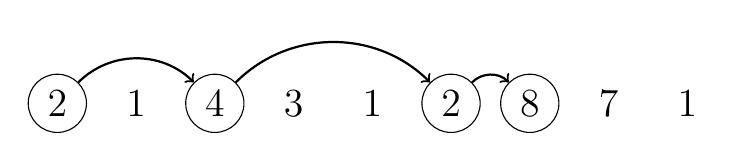
\begin{tikzpicture}

    \tikzstyle{seqc}=[draw, circle]

    \node [seqc] (1) {\Large $2$};
    \node [right of=1, node distance=1cm] (2) {\Large $1$};
    \node [seqc, right of=2, node distance=1cm] (3) {\Large $4$};
    \node [right of=3, node distance=1cm] (4) {\Large $3$};
    \node [right of=4, node distance=1cm] (5) {\Large $1$};
    \node [seqc, right of=5, node distance=1cm] (6) {\Large $2$};
    \node [seqc, right of=6, node distance=1cm] (7) {\Large $8$};
    \node [right of=7, node distance=1cm] (8) {\Large $7$};
    \node [right of=8, node distance=1cm] (9) {\Large $1$};

    \path[->,thick,bend left=45]
        (1) edge (3)
        (3) edge (6)
        (6) edge (7)
        ;
    \end{tikzpicture}
    \end{center}
    \caption{A $2$-sequence.}
\label{3-fig:isequence}
\end{figure}

\Cref{3-fig:isequence} gives an example of a $2$-sequence. The circled
priorities are the indices used in the sequence. Note that there are exactly
$2^2 = 4$ indices used, and that every circled priority is even. Inner
domination is satisfied because every priority that is between two circled
priorities is lower than one of the two end points, and outer domination is
satisfied because the final circled priority $8$ is larger than all the
priorities that come after it.

\paragraph{\bf The relationship to parity games.}
The relationship between $i$-sequences and parity games is explained by the
following lemma.

\begin{lemma}[Completeness for the separating automaton]
\label{3-lem:isequencewin}
Suppose that Adam and Eve play positional strategies in the parity game,
and let $\pi$ the resulting play.
\begin{itemize}
\item If Eve wins the parity game, then there exists prefixes of $\pi$ that
contain arbitrarily long $i$-sequences.
\item If Adam wins the parity game, then no prefix of $\pi$ will contain a
$\lceil \log n \rceil$-sequence.
\end{itemize}
\end{lemma}
\begin{proof}
If Eve wins the parity game then the largest
priority occurring in $\pi$ infinitely often is even. Let $p$ this priority.
To construct a prefix containing an $i$-sequence, we find the first index $j$
after which no priority $q > p$ is seen. We take as our indices $j_1 < j_2 <
\dots < j_{2^i}$ the first $2^i$ occurrences of priority $p$ after index $j$.
Evenness is trivially satisfied, and both inner and outer domination are
satisfied because no priority larger than $p$ is seen after index $j$.

We prove the second claim by contradiction. Suppose that Adam wins the game, but
that there is a prefix of $\pi$ that contains a $\lceil \log n \rceil$-sequence.
Since the sequence indexes $2^{\lceil \log n \rceil} \ge n$ vertices of the
game, it must index the same vertex $v$ twice. Thus our $i$-sequence must
contain a cycle passing through $v$. Note that inner domination ensures that the
largest priority on the cycle that passes through $v$ is even. However, no even
cycle can be formed when Adam wins the game by playing a positional winning
strategy, and so we have arrived at our contradiction.
\end{proof}

To summarise, if Eve wins the game, then she has a strategy that ensures that
arbitrarily long $i$-sequences occur, while if Adam wins the game then he has a
strategy that ensures that no $\lceil \log n \rceil$-sequence occurs. So to
solve the parity game, it is sufficient to determine whether Eve can force a
$\lceil \log n \rceil$-sequence to occur.

\paragraph{\bf A data structure for recognising $i$-sequences.}
We will build a quasi-polynomial sized automaton that reads a sequence of
priorities, 
and determines whether that sequence of priorities contains a
$k$-sequence. 
The automaton is defined by a data structure that we call a \emph{record}, which
contains information about the $i$-sequences that have been seen so far in the
sequence.  

A record is a sequence $b_k, b_{k-1}, \dots, b_1, b_0$, where each
$b_i$ is either a priority, or the special symbol $\siblank$. The value of $b_i$
has the following meaning: 
\begin{itemize}
\item \textbf{Witnessing.} If $b_i \ne \siblank$, then we have seen an
$i$-sequence, and the final priority on that $i$-sequence is $b_i$. 
\item \textbf{Order.} If $b_i \ne \siblank$ and $b_j \ne \siblank$ and $j < i$,
then the first index of the $j$-sequence witnessed by $b_j$ occurs after the
last index of the $i$-sequence witnessed by $b_i$.
\end{itemize}
Note that, although each element $b_i$ records the existence of an
$i$-sequence, the record data structure \emph{does not} store the $2^i$ indices
of this $i$-sequence, it only stores the priority of the final index of that
sequence.

\begin{figure}[!ht]
    \begin{center}
    \begin{tikzpicture}
    \tikzstyle{seqc}=[draw, circle]
    \node [seqc,red] (1) {\Large $2$};
    \node [right of=1, node distance=0.9cm] (2) {\Large $1$};
    \node [seqc, red, right of=2, node distance=0.9cm] (3) {\Large $4$};
    \node [seqc, red, right of=3, node distance=0.9cm] (4) {\Large $2$};
    \node [seqc, red, right of=4, node distance=0.9cm] (5) {\Large $8$};
    \node [right of=5, node distance=0.9cm] (6) {\Large $7$};
    \node [seqc, blue, right of=6, node distance=0.9cm] (7) {\Large $2$};
    \node [right of=7, node distance=0.9cm] (8) {\Large $1$};
    \node [seqc, blue, right of=8, node distance=0.9cm] (9) {\Large $4$};
    \node [right of=9, node distance=0.9cm] (10) {\Large $1$};
    \node [seqc, grey, right of=10, node distance=0.9cm] (11) {\Large $2$};

    \path[->,thick,bend left=45,red]
        (1) edge (3)
        (3) edge (4)
        (4) edge (5)
        ;

    \path[->,thick,bend left=45,blue]
        (7) edge (9)
        ;
    \end{tikzpicture}
    \end{center}
\caption{An example sequence that corresponds to the record $\siblank 8 4 2$.}
\label{3-fig:ds}
\end{figure}

\Cref{3-fig:ds} shows an example sequence that is consistent with the
record that sets $b_3 = \siblank$, $b_2 = 8$, $b_1 = 4$, and $b_0 = 2$.
The red $2$-sequence is represented by $b_2 = 8$, which is the last priority of
the $2$-sequence. The blue $1$-sequence starts after the end of the
$2$-sequence, and it is represented by $b_1 = 4$. Likewise the grey
$0$-sequence starts after the end of the $1$-sequence, and is represented by
$b_0 = 2$. There is no $3$-sequence in the example, and this is represented by
setting $b_3 = \siblank$.

\paragraph{\bf The update rule.}
Suppose that we have a record that represents the $i$-sequences in a
finite sequence of priorities, and that we then read the next priority $p$ in
that sequence. We need to update the record to take this priority into
account. We do this by applying the following \emph{update rule}.
The update rule consists of two steps, which occur one after the other.

\begin{itemize}
\item \textbf{Step 1.} In this step, we find the largest index $i$
such that $b_j$ is even for all $j \le i$. If $b_i = \siblank$, or $b_i < p$,
then we create a new record $b'_k$, $b'_{k-1}$, \dots, $b'_0$ by
setting:
\begin{equation*}
b'_j = \begin{cases}
b_j & \text{if $j > i$,} \\
p & \text{if $j = i$,} \\
\siblank & \text{if $j < i$.} 
\end{cases}
\end{equation*}
If there is no index $i$ that satisfies the conditions, then we do not modify
the record.

\item \textbf{Step 2.} In step 2, we take the output of step 1, and we find the
largest index $i$ such that $p > b_i$ and we create a new record $b'_k$,
$b'_{k-1}$, \dots, $b'_0$ by setting:
\begin{equation*}
b'_j = \begin{cases}
b_j & \text{if $j > i$,} \\
p & \text{if $j = i$,} \\
\siblank & \text{if $j < i$.} 
\end{cases}
\end{equation*}
Again, if there is no such index $i$, then the record is not modified.
\end{itemize}

\begin{figure}[!ht]
    \begin{center}
    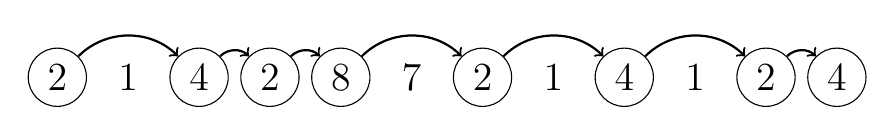
\begin{tikzpicture}
    \tikzstyle{seqc}=[draw, circle]
    \node [seqc] (1) {\Large $2$};
    \node [right of=1, node distance=0.9cm] (2) {\Large $1$};
    \node [seqc, right of=2, node distance=0.9cm] (3) {\Large $4$};
    \node [seqc, right of=3, node distance=0.9cm] (4) {\Large $2$};
    \node [seqc, right of=4, node distance=0.9cm] (5) {\Large $8$};
    \node [right of=5, node distance=0.9cm] (6) {\Large $7$};
    \node [seqc, right of=6, node distance=0.9cm] (7) {\Large $2$};
    \node [right of=7, node distance=0.9cm] (8) {\Large $1$};
    \node [seqc, right of=8, node distance=0.9cm] (9) {\Large $4$};
    \node [right of=9, node distance=0.9cm] (10) {\Large $1$};
    \node [seqc, right of=10, node distance=0.9cm] (11) {\Large $2$};
    \node [seqc, right of=11, node distance=0.9cm] (12) {\Large $4$};
    %\onslide<5>{\node [seq, right of=11, node distance=0.9cm] (12) {\Large
    %$\mathbf{9}$};}

    \path[->,thick,bend left=45]
        (1) edge (3)
        (3) edge (4)
        (4) edge (5)
        (5) edge (7)
        (7) edge (9)
        (9) edge (11)
        (11) edge (12)
        ;

    \end{tikzpicture}
    \end{center}
    \caption{An example of a Step 1 update applied to the sequence and record from~\cref{3-fig:ds}}
\label{3-fig:ds1}
\end{figure}
Intuitively, Step 1 attempts to combine the $i$-sequences in the existing record
into a longer $i$-sequence. Suppose that we have read the sequence shown in~\cref{3-fig:ds}, 
that we have compute the record $\siblank 8 4 2$, and that the next priority in the sequence is $4$.
\Cref{3-fig:ds1} shows the result of applying Step 1 to this situation.
Observe that $3$ is the largest index $i$ such that for all $j < i$ we have that
$b_j$ is even, so Step 1 will output the record $4 \siblank \siblank \siblank$.

So in this circumstance, Step 1 claims that we have now seen a $3$-sequence.
\Cref{3-fig:ds1} shows why this is correct: the $0$-sequence of $b_0$, the
$1$-sequence of $b_1$, and the $2$-sequence of $b_2$ can be merged together,
along with the new priority, to create a $3$-sequence. Observe that inner
domination in this new $3$-sequence is satisfied due to the outer domination
property for each of the $i$-sequences that it was constructed from.
For example, the $2$-sequence ends at priority $8$, and the $1$-sequence begins
at priority $2$, and we know that $8$ must dominate all priorities between the
$8$ and the $2$ because $8$ is required to dominate \emph{all} priorities that
follow it.

\begin{figure}[!ht]
    \begin{center}
    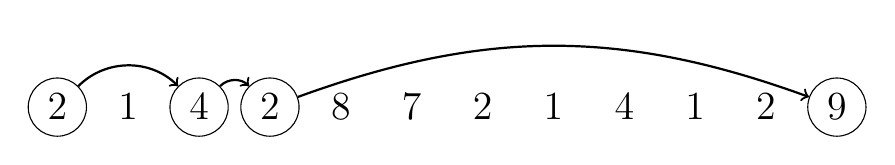
\begin{tikzpicture}
    \tikzstyle{seqc}=[draw, circle]
    \node [seqc] (1) {\Large $2$};
    \node [right of=1, node distance=0.9cm] (2) {\Large $1$};
    \node [seqc, right of=2, node distance=0.9cm] (3) {\Large $4$};
    \node [seqc, right of=3, node distance=0.9cm] (4) {\Large $2$};
    \node [right of=4, node distance=0.9cm] (5) {\Large $8$};
    \node [right of=5, node distance=0.9cm] (6) {\Large $7$};
    \node [right of=6, node distance=0.9cm] (7) {\Large $2$};
    \node [right of=7, node distance=0.9cm] (8) {\Large $1$};
    \node [right of=8, node distance=0.9cm] (9) {\Large $4$};
    \node [right of=9, node distance=0.9cm] (10) {\Large $1$};
    \node [right of=10, node distance=0.9cm] (11) {\Large $2$};
    \node [seqc, right of=11, node distance=0.9cm] (12) {\Large $9$};
    %\onslide<5>{\node [seq, right of=11, node distance=0.9cm] (12) {\Large
    %$\mathbf{9}$};}

    \path[->,thick,bend left=45]
        (1) edge (3)
        (3) edge (4);

    \path[->,thick,bend left=20]
        (4) edge (12)
        %(5) edge (7)
        %(7) edge (9)
        %(9) edge (11)
        %(11) edge (12)
        ;

    \end{tikzpicture}
    \end{center}
    \caption{An example of a Step 2 update applied to the sequence and record from~\cref{3-fig:ds}}
\label{3-fig:ds2}
\end{figure}

Step 2 ensures that the outer domination property holds. 
In~\cref{3-fig:ds2}, we show the result of applying Step 2 to the record
$\siblank 8 4 2$ that corresponds to the sequence shown in~\cref{3-fig:ds},
when the next priority in the sequence is $9$. Observe that since $9 > 8$, the
outer domination property for the $2$-sequence ending at $8$ now fails to hold,
and likewise for the sequences ending at $4$ and $2$. Hence, Step 2 deletes the
$0$-sequence and $1$-sequence from the record, and updates the $2$-sequence to
end at $9$, thereby restoring outer domination. The resulting record is $\siblank
9 \siblank \siblank$.

\paragraph{\bf Correctness.} 
To compute a record for a particular sequence of priorities, we start with the
record $\siblank \siblank \dots \siblank$, and then process the sequence one
priority at a time, using the update rule that we have described. 

We must now argue that the record data structure and update rule is sufficient
to decide the winner of a parity game. The following lemma states that a record
will never falsely claim that an $i$-sequence has occurred.

\begin{lemma}[Correctness for the separating automaton]
\label{3-lem:correctness_separating_automata}
Let $b_k, b_{k-1}, \dots, b_0$ the record for a sequence of priorities $\pi$.
If $b_i \ne \siblank$, then $\pi$ contains an $i$-sequence.
\end{lemma}
\begin{proof}
This can be proved by induction over the components of the record. In fact we
will prove the slightly stronger order property that we mentioned earlier:
the $i$-sequence corresponding to
$b_i$ starts after the $j$ sequence corresponding to $b_j$ whenever $i < j$ and
$b_i \ne \siblank$ and $b_j \ne \siblank$.

The base case is trivially true, since the value of $b_0$ asserts the existence
of a 0-sequence, and any priority by itself is a $0$-sequence. So when Step 1 or
Step 2 updates $b_0$, the corresponding $0$-sequence is the new priority, and
this clearly starts after all other $i$-sequences in the record.

For the inductive step, we must prove that the two steps of the update rule are
correct. 
\begin{itemize}
\item For Step 1 updates, we can use the inductive hypothesis to argue that, for
each $j < i$, the $j$-sequence corresponding to $b_j$ exists, and that they
appear in order in the sequence, and that it ends before the sequence
corresponding to $b_{j-1}$ starts. Furthermore, the outer domination property
the $j$-sequence ensures that all priorities between the end of the
$j$-sequence and the start of the $(j-1)$-sequence are dominated by the last
priority in the $j$-sequence, which must be even according to the definition of
a Step 1 update.
Hence, we can combine all of the $j$-sequences with $j < i$ together, along with
the new priority, to create an $i$-sequence. This new $i$-sequence starts at
exactly the same point as the sequence corresponding to $b_{i-1}$, and so the
order property still holds.

\item For Step 2 updates, we only need to argue that the value of $b'_i$
correspond to an $i$ sequence. This can be constructed as we showed in~\cref{3-fig:ds2}: 
take the $i$-sequence that corresponds to $b_i$, and
replace the final priority with the new priority. Observe that the final
priority of an $i$-sequence is permitted to be odd, and so this new sequence
satisfies all of the requirements of an $i$-sequence. Furthermore, the starting
point of this sequence has not changed, and so the order property is preserved.
\end{itemize}
\end{proof}

As a consequence of the lemma above, if Adam has a strategy to ensure that no
$k$-sequence occurs in the game, then Adam has a strategy to ensure that the
$b_k$ component of the record is never set so that $b_k \ne \siblank$.

It can be shown that the other direction is also true: if an $i$-sequence has
occurred, then there will be some index $j \ge i$ such that $b_j \ne \siblank$.
However, the proof is somewhat tedious, and this statement is actually stronger
than what we need. To argue that the record can determine the winner of a parity
game, the following weaker lemma suffices. 

\begin{lemma}[Weaker correctness for the separating automaton]
\label{3-lem:weaker_correctness_separating_automaton}
Let $\pi$ an infinite play that is winning for Eve. For all $k$, there exists
a prefix of $\pi$ such that $b_k \ne \siblank$.
\end{lemma}
\begin{proof}
Let $p$ the largest even priority that is seen infinitely often, and let $j$
be the first index after which no priority larger than $p$ is visited. We argue
that after index $j$ has been reached, the record will eventually set $b_i \ne
\siblank$ for all $i$.

To see why, observe that after index $j$ has been reached, Step 2 cannot replace
any component $b_j$ with $b_j = p$, since Step 2 can only overwrite the priority
in $b_j$ when the new priority $p'$ satisfies $p' > b_j$, but no priority $p' >
p$ is seen after index~$j$. 

On the other hand, Step 1 will always be triggered whenever we visit the
priority $p$. Step 1 will always set some component of the record to $p$, and as
we have observed this cannot be overwritten by Step 2. Moreover, since $p$ is
even, repeated application of Step 1 will
build a longer and longer $i$-sequences whose outer domination
priority is $p$. Thus, after we have made $2^k$ visits to $p$, we will have set
$b_k = p \ne \siblank$, if we have not done so already.
\end{proof}

Hence, if Eve wins the parity game, then she has a strategy to eventually ensure
that $b_k \ne \siblank$. Combining the two lemmas above, with~\cref{3-lem:isequencewin} gives the following corollary.

\begin{corollary}[Correctness of the reduction for the separating automaton]
\label{3-cor:correctness_reduction_separating_automaton}
Suppose that we monitor the play of a parity game with a record $b_{\lceil \log
n \rceil}, \dots, b_0$. Eve has a strategy that ensures $b_{\lceil \log n
\rceil} \ne \siblank$ if and only if Eve wins the parity game.
\end{corollary}

\paragraph{\bf The size of the automaton.}
The record data structure and update rule can be encoded as a deterministic
finite automaton that reads the play. Each state of the automaton is associated
with some configuration of $b_{\lceil \log n \rceil}, \dots, b_0$, and the
transitions of the automaton are defined by the update rule. 

This automaton has quasipolynomial size. The number of states used in the
automaton is the number of possible configurations of
$b_{\lceil \log n \rceil}, \dots, b_0$. Each $b_i$ can be one of the $d$
priorities in the game, or the symbol $\siblank$, and so there are $d + 1$
possible values that it can take. Moreover there are $\log n + 1$ components of
the record, so the total number of configurations is at most
$(d+1)^{\log n +1} = n^{O(\log d)}$.



%%%%%%%%%%%%%%%%%%
%%%%%%%%%%%%%%%%%%
%%%%%%%%%%%%%%%%%%

\section{A quasipolynomial time value iteration algorithm}
\label{3-sec:value_iteration}
In this section and the next we discuss two families of fixed point algorithms for solving games.
The goal is to highlight the main ingredients for constructing algorithms in these two families.
If the descriptions below are too abstract it may be useful to see concrete instantiations: 
we refer to \cref{4-chap:payoffs} for archetypical examples, and also to \cref{3-chap:parity}.

\subsection*{The value function}
The key ingredient of a value iteration algorithm is a value function.
For a quantitative game $\Game$ with condition $f = \Phi[\col]$ over the set of colours $C$, 
assuming that $\Game$ is determined it admits a value function
\[
\Value^{\game} : V \to \Rinfty,
\]
which is defined as 
\[
\Value^{\game} = \sup_{\sigma}\ \inf_{\tau}\ f(\pi_{\sigma,\tau}^v) = \inf_{\tau}\ \sup_{\sigma}\ f(\pi_{\sigma,\tau}^v),
\]
where $\sigma$ ranges over strategies of Eve, $\tau$ over strategies of Adam, 
and $\pi_{\sigma,\tau}^v$ is the play consistent with $\sigma$ and $\tau$ from $v$.
In particular we write $\Value^{\sigma}$ for $\inf_{\tau}\ f(\pi_{\sigma,\tau}^v)$.

For a qualitative game $\Game$ there is no notion of a value function so the first step in constructing a value iteration
algorithm is to define a meaningful notion of value function.
Let us assume that the condition is $\Omega[\col]$ over the set of colours $C$.
The first ingredient is a lattice $(Y,\le)$ together with a function $\val : C^\omega \to Y$ for evaluating plays, taking the role of the quantitative condition $f$.
The value function is $\Value^{\game} : V \to Y$ defined as
\[
\Value^{\game}(v) = \sup_{\sigma}\ \inf_{\tau}\ \val(\pi_{\sigma,\tau}^v).
\]
As above we write $\Value^{\sigma}$ for $\inf_{\tau}\ \val(\pi_{\sigma,\tau}^v)$.

The following principle implies that computing the value function in particular yields the winning regions.

\begin{principle}[Characterisation of the winning regions]
For all vertices $v$ we have that Eve wins from $v$ if and only if $\Value^{\game}(v) \neq \bot$, where $\bot$ is the least element in $Y$.
\end{principle}

In the remainder of this section we assume the existence of a value function $\Value^{\game} : V \to Y$ (note that choosing $Y = \Rinfty$ covers the quantitative case) and fix as a goal to either compute or approximate it.

\subsection*{Fixed point}
We let $F_V$ denote the set of functions $V \to Y$, it is a lattice when equipped with the componentwise (partial) order induced by $Y$:
we say that $\mu \le \mu'$ if for all vertices $v$ we have $\mu(v) \le \mu'(v)$.

The second ingredient is a function $\delta : Y \times C \to Y$ inducing an operator $\Op : F_V \to F_V$ defined by\footnote{This form is for two player games, the operator has to be adapted to more complex settings such as stochastic or concurrent games.} and satisfying the following principle:
\[
\Op(\mu)(v) = 
\begin{cases}
\max \set{\delta( \mu(v'), \col(v)) : (v,v') \in E} & \text{ if } v \in \VE, \\
\min \set{\delta( \mu(v'), \col(v)) : (v,v') \in E} & \text{ if } v \in \VA.
\end{cases}
\]

\begin{principle}[Fixed point]
The function $\val^{\game}$ is a fixed point of the operator $\Op$.
\end{principle}
This fixed point principle is often tightly related to the fact the $\Game$ is positionally determined for both players.
The fact that $\val^{\game} = \Op(\val^{\game})$ means that from a vertex $v$, 
the value $\val^{\game}(v)$ can be computed locally, \textit{i.e.} by considering the maximum or the minimum over all edges $(v,v')$ 
of a function $\delta$ of $\val^{\game}(v')$ and of $\col(v)$.
The choice of minimum or maximum corresponds to the goal of the players: Eve wants to maximise the outcome and Adam to minimise it.

\subsection*{Fixed point through contraction}
Let us first consider the family of value iteration algorithms based on Banach's fixed point theorem as stated in \cref{1-thm:banach}
and let us fix as a goal to approximate $\Value^{\game}$.
We equip $F_V$ with a norm $||\cdot||$.

\begin{principle}[Fixed point through contraction]
The operator $\Op$ is contracting in the complete space $(F_V,||\cdot||)$ implying that $\Value^{\game}$ is the unique fixed point of $\Op$.
\end{principle}

The algorithm is the following:
we choose some $\Value_0 : V \to Y$ and then compute the sequence $(\Value_k)_{k \in \N}$ defined by $\Value_{k+1} = \Op(\Value_k)$
until we get the desired quality of approximation for $\Value^{\game}$.
We have
\[
||\Value_k - \Value^{\game}|| \le \frac{\lambda^k}{1 - \lambda} \cdot ||\Value_1 - \Value_0||,
\]
where $\lambda \in (0,1)$ is the contraction factor of $\Op$.
Hence to get an $\varepsilon$-approximation of $\Value^{\game}$ it is enough to perform 
$k = O \left( \frac{\log(\varepsilon)}{\log(\lambda)} \right)$ iterations.

\subsection*{Fixed point through monotonicity}
The second family of algorithms is based on Kleene's fixed point theorem as stated in \cref{1-thm:kleene}.

\begin{principle}[Fixed point through monotonicity]
The function $\delta$ is monotonic (meaning that if $y \le y'$ then for all colours $c$ we have $\delta(y,c) \le \delta(y',c)$)
and $\val^{\game}$ is the greatest fixed point of the monotonic operator $\Op$.
\end{principle}

\begin{remark}
It is possible to define the value function as the \textit{least} fixed point of $\Op$, 
and this is equivalent up to some inversions in the lattice $(Y,\le)$ and the operator~$\Op$.
There are two reasons why we chose to define the value function as the \textit{greatest} fixed point of $\Op$.
The first is that this implies that the operator $\Op$ is defined in the same way in both qualitative and quantitative cases (for the other definition, min and max would be swapped in the definition of $\Op$ for qualitative games, which contradicts the intuition given above),
and the second is that with this convention losing from $v$ is equivalent to $\Value^{\game}(v) = \bot$,
while in the other convention it is equivalent to $\Value^{\game}(v) = \top$, where $\top$ is the greatest element in $Y$.
\end{remark}

\Cref{1-thm:kleene} states that $\Value^{\game}$ is also the greatest post-fixed point.
Recall that a post-fixed point is $\mu$ such that $\mu \le \Op(\mu)$, which in this context we call a ""progress measure"".
Expanding the definitions: for all vertices $v$, we have
\[
\begin{array}{llll}
\mu(v) & \le & \max \set{\delta( \mu(v'), \col(v)) : (v,v') \in E} & \text{ if } v \in \VE, \\
\mu(v) & \le & \min \set{\delta( \mu(v'), \col(v)) : (v,v') \in E} & \text{ if } v \in \VA,
\end{array}
\]
which is equivalent to the more familiar definition of progress measures: for all vertices $v$, we have
\[
\begin{array}{llll}
\exists (v,v') \in E,\ & \mu(v) \le \delta( \mu(v'), \col(v)) & \text{ if } v \in \VE, \\
\forall (v,v') \in E,\ & \mu(v) \le \delta( \mu(v'), \col(v)) & \text{ if } v \in \VA.
\end{array}
\]
The characterisation principle can be equivalently stated as follows.

\begin{principle}[Characterisation of the winning regions -- equivalent formulation with progress measures]
For all vertices $v$ we have Eve wins from $v$ if and only if there exists a progress measure $\mu$ such that $\mu(v) \neq \bot$.
\end{principle}

The third information given by \cref{1-thm:kleene} is that $\Value^{\game}$ is the limit of the sequence $(\Op^k(\top))_{k \in \N}$.

If $Y$ is a finite lattice then so is $F_V$, and the algorithm for computing $\Value^{\game}$ is as follows:
we let $\Value_0$ defined by $\Value_0(v) = \top$ and then compute the sequence $(\Value_k)_{k \in \N}$ defined by 
$\Value_{k+1} = \min(\Op(\Value_k), \Value_k)$.
There exists $k$ such that $\Value_{k+1} = \Value_k$, at which point we have that $\Value_k = \Value^{\game}$,
from which we obtain the winning regions thanks to the characterisation principle.
A naive upper bound on $k$ is $|F_V| \le |Y|^n$, but usually a finer analysis of the algorithm yields better bounds on the number of iterations to reach the fixed point.

If $Y$ is not finite that the sequence $(\Value_k)_{k \in \N}$ converges towards $\Value^{\game}$ and further analysis is required to evaluate the convergence speed.

\begin{remark}
It is sometimes useful to define instead of the operator $\Op$ a set of operators $(\Op_v)_{v \in V}$:
\[
\Op_v(\mu)(u) = 
\begin{cases}
\mu(v) & \text{ if } u \neq v, \\
\max \set{\delta( \mu(v'), \col(v)) : (v,v') \in E} & \text{ if } u = v \in \VE, \\
\min \set{\delta( \mu(v'), \col(v)) : (v,v') \in E} & \text{ if } u = v \in \VA.
\end{cases}
\]
The fixed points of $\Op$ and of the set of operators $(\Op_v)_{v \in V}$ are the same
and the ideas described above can be applied using \cref{1-thm:kleene_set_operators} instead of \cref{1-thm:kleene}.
\end{remark}


%%%%%%%%%%%%%%%%%%
%%%%%%%%%%%%%%%%%%
%%%%%%%%%%%%%%%%%%

\section{Comparing the three families of algorithms}
\label{3-sec:relationships}
At the beginning of the chapter we described three families of algorithms: 
strategy improvement, attractor decomposition, and value iterations.

\vskip1em
Let us first clarify the relationship between the separation framework discussed in \cref{3-sec:separation}
and the value iteration paradigm presented in \cref{3-sec:value_iteration}.
Both are families of algorithms: 
\begin{itemize}
	\item An $(n,d)$-separating automaton $\Automaton$ induces an algorithm for solving parity games in time 
$O(m \cdot |\Automaton|)$ where $|\Automaton|$ is the size of $\Automaton$, meaning the number of states.
	\item An $(n,d/2)$-universal tree $T$ induces a value iteration algorithm for solving parity games in time 
proportional to $|T|$ where $|T|$ is the size of $T$, meaning the number of leaves (the exact complexity depends on the cost of computing $\delta$ in $T$, which is typically small).
\end{itemize}
These two families are in a strong sense equivalent:

\begin{theorem}\hfill
\begin{itemize}
	\item An $(n,d)$-separating automaton induces an $(n,d/2)$-universal tree of the same size;
	\item An $(n,d/2)$-universal tree induces an $(n,d)$-separating automaton of the same size.
\end{itemize}
\end{theorem}
We do not prove this theorem here but note that it can be stated more generally for any positionally determined objective,
replacing universal trees by the notion of universal graphs.

The main advantage of the value iteration presentation is the space complexity, which for a good choice of the universal tree
can be made very small (quasilinear).

\vskip1em
In terms of complexity, the strategy improvement has exponential complexity, while both attractor decompositions and value iterations algorithms have quasipolynomial complexity.
Let us make a finer comparison: the complexity of the attractor decomposition algorithm is a polynomial multiplied by the (non polynomial) term
\[
\binom{\lceil \log(n) \rceil + d - 1}{\lceil \log(n) \rceil},
\]
while for the value iteration algorithm the complexity is a polynomial multiplied by the (also non polynomial) term
\[
\binom{\lceil \log(n) \rceil + d/2 - 1}{\lceil \log(n) \rceil}.
\]
The key difference is that the former performs an induction using all priorities, while the latter considers only odd priorities hence the dependence in $d/2$.
Although our presentation of the attractor decomposition algorithm does not make it explicit, 
this class of algorithms is also related to the notion of universal trees; 
however an algorithm is induced not by one $(n,d/2)$-universal tree, but by two: one for each player,
which are then interleaved to organise the recursive calls of the algorithm.

\vskip1em
Since both value iteration and attractor decomposition algorithms are connected to the combinatorial notion of universal trees,
the next question is whether the construction given in \cref{3-sec:value_iteration} is optimal.
The answer is unfortunately yes, there exists a lower bound on the size of universal trees which matches this construction up to polynomial factors.

\vskip1em
The last question we discuss here is whether there exists a quasipolynomial strategy improvement algorithm.
In particular a natural attempt would be to use universal trees for this endeavour.
Unfortunately, this fails: \cref{3-lem:key_property} explains that for the particular choice of the lattice $Y$,
functions $\mu : V \to Y$ can be used both to certify that a graph satisfies parity or that it satisfies the complement of parity.
Both implications are used in the correctness proof of the algorithm.
This symmetric feature is lost with universal trees, which only satisfy one of the two implications, stated in \cref{3-lem:progress_measure}.


%%%%%%%%%%%%%%%%%%
%%%%%%%%%%%%%%%%%%
%%%%%%%%%%%%%%%%%%

\section*{Bibliographic references}
\label{3-sec:references}
We refer to~\cref{2-sec:references} for the role of parity objectives and how they emerged in automata theory as a subclass of Muller objectives.
Another related motivation comes from the works of Emerson, Jutla, and Sistla~\cite{Emerson&Jutla&Sistla:1993},
who showed that solving parity games is linear-time equivalent to the model-checking problem for modal $\mu$-calculus.
This logical formalism is an established tool in program verification, and a common denominator to a wide range of modal, temporal and fixpoint logics used in various fields.

\vskip1em
Let us discuss the progress obtained over the years for each of the three families of algorithms.

\vskip1em
\textit{Value iteration algorithms and separating automata}.
The heart of value iteration algorithms is the value function, which in the context of parity games and related developments for automata
have been studied under the name progress measures or signatures.
They appear naturally in the context of fixed point computations so it is hard to determine who first introduced them.
Streett and Emerson~\cite{Streett&Emerson:1984,Streett&Emerson:1989} defined signatures for the study of the modal $\mu$-calculus,
and Stirling and Walker~\cite{Stirling&Walker:1989} later developped the notion.
Both the proofs of Emerson and Jutla~\cite{Emerson&Jutla:1991} and of Walukiewicz~\cite{Walukiewicz:1996} use signatures to show the positionality of parity games over infinite games.

Jurdzi{\'n}ski~\cite{Jurdzinski:2000} used this notion to give the first value iteration algorithm for parity games, 
with running time $O(m n^{d/2})$.
The algorithm is called ``small progress measures'' and is an instance of the class of value iteration algorithms we construct 
in~\cref{3-sec:value_iteration} by considering the universal tree of size $n^h$.
Bernet, Janin, and Walukiewicz~\cite{Bernet&Janin&Walukiewicz:2002} investigated reductions from parity games to safety games
through the notion of permissive strategies, and constructed a separating automaton\footnote{We note that the general framework of separating automata came later, introduced by Boja{\'n}czyk and Czerwi{\'n}ski~\cite{Bojanczyk&Czerwinski:2018}.} corresponding to the universal tree of size $n^h$.

The new era for parity games started in 2017 when Calude, Jain, Khoussainov, Li, and Stephan~\cite{Calude&Jain&al:2017} constructed a quasipolynomial time algorithm. 
Our presentation follows the technical developments of the subsequent paper by Fearnley, Jain, Schewe, Stephan, and Wojtczak~\cite{Fearnley&Jain&al:2017} which recasts the algorithm as a value iteration algorithm.
Boja{\'n}czyk and Czerwi{\'n}ski~\cite{Bojanczyk&Czerwinski:2018} introduce the separation framework to better understand the original algorithm.

Soon after two other quasipolynomial time algorithms emerged.
Jurdzi{\'n}ski and Lazi{\'c}~\cite{Jurdzinski&Lazic:2017} showed that the small progress measure algorithm can be adapted to a ``succinct progress measure'' algorithm, matching (and slightly improving) the quasipolynomial time complexity.
The presentation using universal tree that we follow in~\cref{3-sec:value_iteration} and an almost matching lower bound on their sizes is due to Fijalkow~\cite{Fijalkow:2018}.
The connection between separating automata and universal trees was shown by Czerwi{\'n}ski, Daviaud, Fijalkow, Jurdzi{\'n}ski, Lazi{\'c}, and Parys~\cite{Czerwinski&Daviaud&al:2018}. 

The third quasipolynomial time algorithm is due to Lehtinen~\cite{Lehtinen:2018}.
The original algorithm has a slightly worse complexity ($n^{O(\log(n))}$ instead of $n^{O(\log(d))}$),
but Parys~\cite{Parys:2020} later improved the construction to (essentially) match the complexity of the previous two algorithms.
Although not explicitly, the algorithm constructs an automaton with similar properties as a separating automaton,
but the automaton is non-deterministic.
Colcombet and Fijalkow~\cite{Colcombet&Fijalkow:2019} revisited the link between separating automata and universal trees
and proposed the notion of good for small games automata, capturing the automaton defined by Lehtinen's algorithm.
The equivalence result between separating automata, good for small games automata, and universal graphs, holds for any positionally determined objective, giving a strong theoretical foundation for the family of value iteration algorithms.

\vskip1em
\textit{Attractor decomposition algorithms}.
The McNaughton Zielonka's algorithm has complexity $O(m n^d)$.
Parys~\cite{Parys:2019} constructed the fourth quasipolynomial time algorithm as an improved take over McNaughton Zielonka's algorithm.
As for Lehtinen's algorithm, the original algorithm has a slightly worse complexity ($n^{O(\log(n))}$ instead of $n^{O(\log(d))}$).
Lehtinen, Schewe, and Wojtczak~\cite{Lehtinen&Schewe&Wojtczak:2019} later improved the construction.
As discussed in~\cref{3-sec:relationships} the complexity of this algorithm is quasipolynomial and of the form $n^{O(\log(d))}$,
but a bit worse than the three previous algorithms since the algorithm is symmetric and has a recursion depth of $d$,
while the value iteration algorithms only consider odd priorities hence replace $d$ by $d/2$.

Jurdzi{\'n}ski and Morvan~\cite{Jurdzinksi&Morvan:2020} constructed a generic McNaughton Zielonka's algorithm parameterised by the choice of two universal trees, one for each player.
\mynote{CONTINUE}


\vskip1em
\textit{Strategy improvement algorithms}.
As we will see in~\cref{4-chap:payoff}, parity games can be reduced to mean payoff games,
so any algorithm for solving mean payoff games can be used for solving parity games.
In particular, the existing strategy improvement algorithm for mean payoff games can be run on parity games. 
V{\"o}ge and Jurdzin{\'n}ski~\cite{Voge&Jurdzinski:2000} introduced the first discrete strategy improvement for parity games,
running in exponential time.
For some time there was some hope that the strategy improvement algorithm, for some well chosen policy on switching edges,
solves parity games in polynomial time.
Friedmann~\cite{Friedmann:2011} cast some serious doubts by constructing numerous exponential lower bounds applying to different variants of the algorithm.
Fearnley~\cite{Fearnley:2017} investigated efficient implementations of the algorithm, focussing on the cost of computing and updating the value function for a given strategy.
Our proof of correctness is original. \mynote{SAY MORE?}

The complexity was reduced to subexponential with randomised algorithms 
by Jurdzin{\'n}ski, Paterson, and Zwick~\cite{Jurdzinski&Paterson&Zwick:2008}.
A natural question is whether there exists a quasipolynomial strategy improvement algorithm; 
as discussed in~\cref{3-sec:relationships} the notion of universal trees cannot be used to achieve this,
and the question remains to this day open.




